\chapter{Resolving a Conducting Conformation of CFTR Using Free Energy Calculations}
\label{chap:opening}
\setcounter{figure}{0}
\renewcommand{\thefigure}{\arabic{chapter}.\arabic{figure}}
\chapquote{You wanna fight?} {- Zachary Picker. Layperson. (personal communication)}


\section*{\centering Abstract} 
The misfunction of the CFTR gene causes Cystic Fibrosis. The protein must conduct both chloride and bicarbonate in order to avoid disease. The recent development of small molecules known as potentiators has demonstrated the clinical efficacy of modulating the CFTR protein such that it occupies an open conformation to relieve disease symptoms. Hence, determining the precise mechanism behind ion conduction through CFTR has important implications for ongoing drug discovery efforts.

Existing atomic structures of CFTR leave unresolved questions behind the conduction mechanism, as these structures exhibit constrictions smaller than the ions themselves. This indicates that there must be some conformational changes to this structure for ions to pass through CFTR. Here we present innovative simulation techniques which combine unbiased molecular dynamics, principal component analysis, OPES-Metadynamics and umbrella sampling to resolve the conduction pathway through the selectivity filter of human CFTR. Our proposed open structure is in better agreement with both theoretical predictions and experimental measurements of the pore architecture of CFTR. We also propose electrophysiology experiments to experimentally test whether this conformation is physiologically accessible.  

The findings of this study demonstrate that computational power and protein forcefields are now sufficiently developed to take advantage of the large database of protein structures collected through the cryo-EM ``resolution revolution" and AI based protein structure predictions. In this era of structural abundance MD based methods can now be used elucidate even more of the protein conformational landscape. This signals an exciting future for computational structural biology and biophysics.

\section{Introduction}

Ion channels are crucial to many cellular functions. When they misfunction, they may cause pain or disease \cite{kingwell2019, kim2014}. Hence, they have been pursed as targets for drugs and the molecular basis for their conduction of ions has been studied closely for some time \cite{santos2017, doyle1998, roux1993}.

One of the most well-known ``channelopathies" is caused by loss-of function mutations in an anion channel, the Cystic Fibrosis Transmembrane conductance Regulator (CFTR). This misfunction leads to Cystic Fibrosis (CF) \cite{riordan1989,gadsby2006}. This is a fatal genetic condition which afflicts an estimated 162000 people worldwide, with a significant number of people unable to access treatment \cite{guo2022}.

The function of mutant CFTR can be restored by molecules known as CFTR modulators. A kind of CFTR modulator known as potentiators interact directly with CFTR to cause it to favor its open, conducting conformation \cite{liu2019}. In current cryo-EM structures of CFTR, there is a constriction along the ion conduction pathway which is too small to allow the ions to pass \cite{zhang2018} (Figure \ref{constricted_sel_filter}A). Hence, the full conduction pathway of ions through CFTR is not yet understood. To understand and improve these drugs, a molecular understanding of the conduction of ions through CFTR is critical. 

The ion permeation pathway of CFTR can be split into two sections. The inner vestibule and the selectivity filter. We have previously studied the motion of chloride through the inner vestibule in chapter \ref{chap:R352Q} \cite{wong2022a}, and in this chapter we will study conduction through the selectivity filter.

The selectivity filter can also be divided into two parts. A lower ``conductivity selectivity filter" and a higher ``permeability filter" (Figure \ref{constricted_sel_filter}B). The different sections in the selectivity filter were characterised by measuring the permeation profiles of different anions under different mutations \cite{linsdell2016}. 

The lower ``conductivity selectivity filter" appears to bind anions as they move through the channel while the ``permeability selectivity filter" is narrow and hydrophobic, so anions do not bind strongly in this region. This is thought to be the origin of the lyotropic sequence of anion selectivity as F337A and L102A in the permeability selectivity filter abolish some level of anion selectivity (Figure \ref{constricted_sel_filter}B) \cite{linsdell2021}. 

\begin{figure}
	\begin{center}
		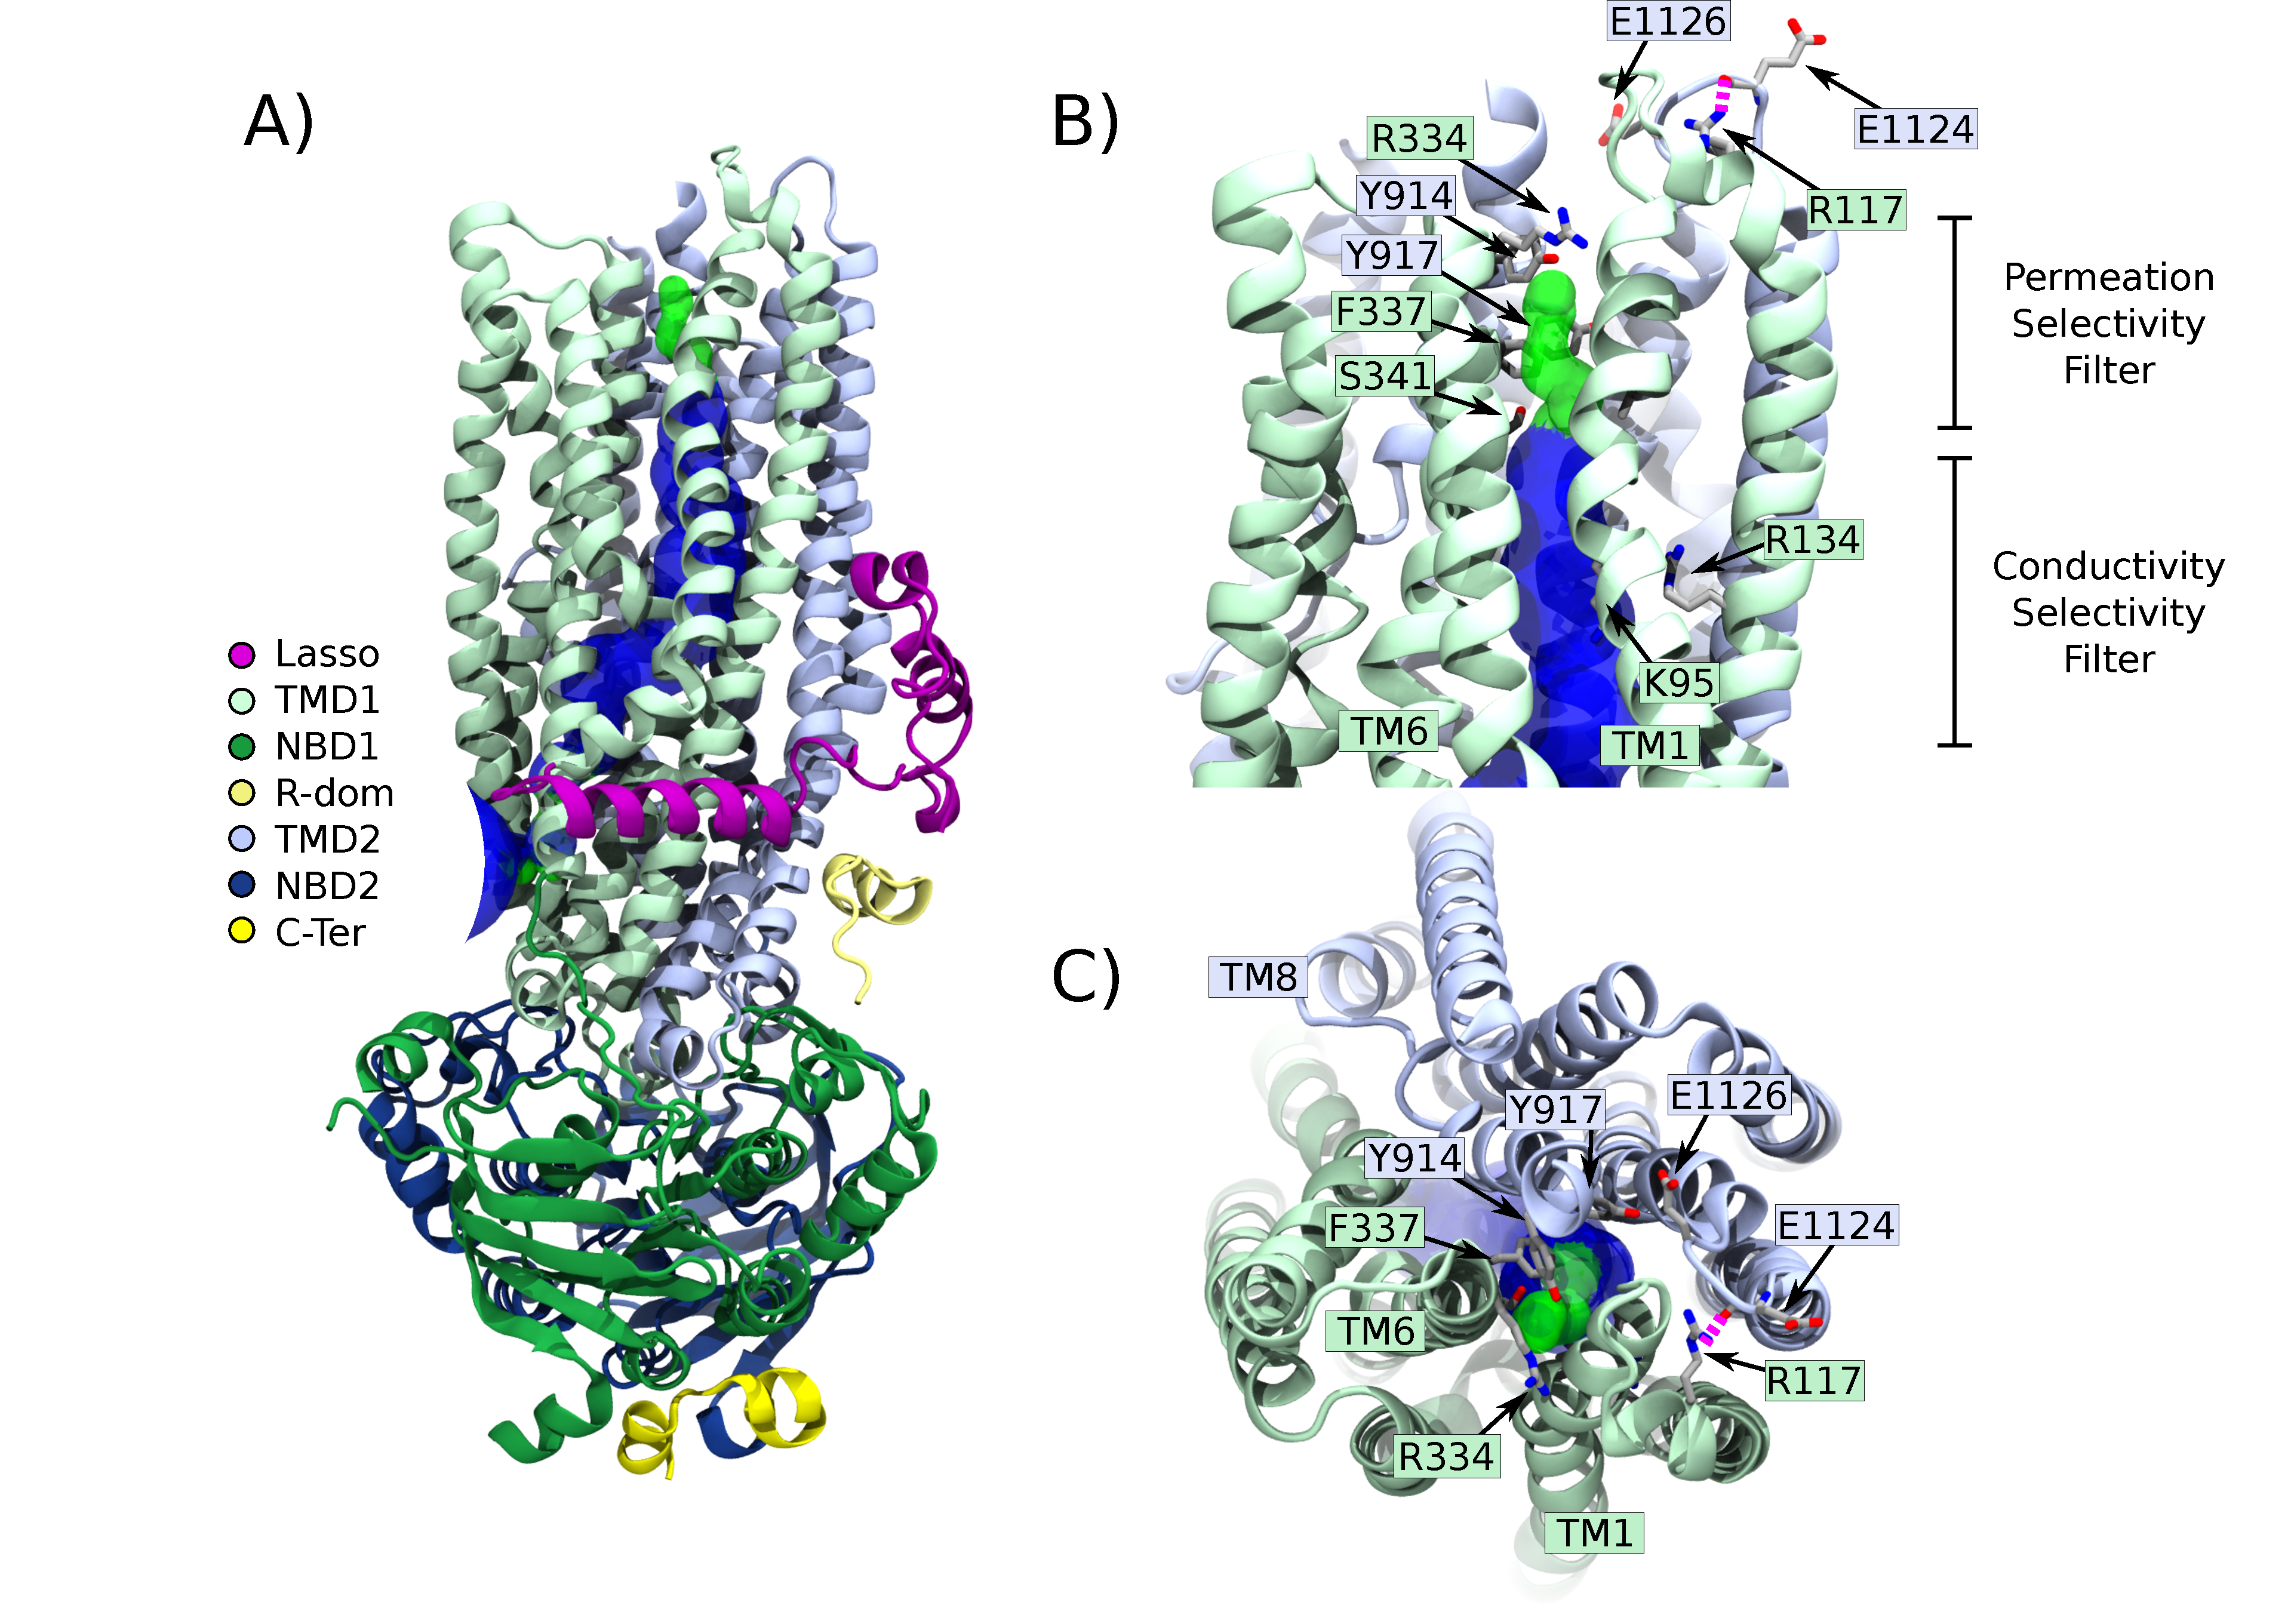
\includegraphics[width=1\textwidth]{figures/opening/overall_hole_constricted.pdf}
	\end{center}
	\captionsetup{singlelinecheck = false, justification=raggedright}
	\caption[Constriction in Cryo-EM Structure (6MSM)] {\textbf{Constriction in Cryo-EM Structure (6MSM)}}{The most recent experimentally resolved structure of hCFTR bound to ATP has a constriction smaller than the radius of chloride ions \cite{zhang2018}. The purpose of this study is to discover a dilated, conducting conformation of CFTR by using this cryo-EM structure as a starting point. A) The constriction occurs between TM1 and 6 on TMD1. The space filling probe is colored blue when a hydrated ion may pass, while it turns green when the ion must be dehydrated. The probe truncates when it encounters a constriction smaller than an ion.  B) Close up of the constriction. Observe how the constriction begins at S341 in the permeability filter and ends at R334 where there is no available space to pass. This leads us to believe that movements in TM6 will help the channel to open. C) A top down view of the selectivity filter. Observe how the architecture of TM1 and TM6 have resulted in a constriction around the conduction pathway.}
	\label{constricted_sel_filter}
\end{figure}

Due to the importance of the conductance of this channel in disease pathology, a molecular understanding behind the basis of its conductivity will inform future efforts in drug design and improve patient outcomes. Unfortunately, current structures of CFTR are insufficiently dilated in order to conduct anions \cite{zhang2018, liu2019, fiedorczuk2022}. They exhibit a constriction smaller than chloride ions themselves (Figure \ref{constricted_sel_filter}C).

The motion of chloride through the selectivity filter has been studied in two \textit{in silico} studies to date \cite{farkas2020, zeng2021}. In the first computational study, performed on zebrafish CFTR (PDB ID: 5W81) \cite{zhang2017a}, metadynamics was used to push chloride around the CFTR selectivity filter, to resolve the conduction pathway. The pathway analysed appears to agree with \textit{in vitro} studies of the selectivity filter in human CFTR \cite{linsdell2016}. However these MetaD calculations exhibited a significant energy barrier to the passage of chloride (roughly 10 kcal/mol) \cite{farkas2020}. This sizeable energetic barrier would appear to conflict with experimental measurements of the channel's conductivity, and indicates that the tested protein conformation is not sufficiently open to readily conduct ions. 

For the second study, hCFTR was studied with a strong applied electric field in MD simulations \cite{zeng2021}. These authors were able to observe the permeation of chloride ions through the channel. However, the number of conduction events these authors observed would imply a conductivity of 0.54 pS (17 events in 10 $\mu$s of sampling at a substantial 500mV bias). This conductivity is an order of magnitude below the experimentally measured conductivity of CFTR (6-10pS) \cite{gong2004, lee2007, linsdell2001, sheppard1999}. These two studies indicate that there are conformational states of CFTR, not yet experimentally visualised, which will support the conduction of chloride and other anions. 

These prior MD studies have focussed on the conduction of chloride, since it is the most physiologically important species to permeate through CFTR. However, it is one of the smallest ions which can pass through CFTR. Larger ions such as bicarbonate and glutathione also move through the channel and their failure to do so plays an important role in disease pathology \cite{gao1999, kogan2003, linsdell1998, tang2009, larusch2014, jun2016}. Hence, it is clear that there is a need to move beyond the available cryo-EM structures of CFTR, to resolve a conducting conformation which may support the passage of larger anions as well as chloride. Here we will present \textit{in silico} methods to compliment this existing structural information and move beyond the available structures of CFTR. 

An \textit{in silico} attempt at this has been made previously, by constructing a model based on zCFTR (PDB ID: 5W81 \cite{zhang2017a}) and steering it toward the outward facing conformation of a distantly related ABC transporter, SAV1866 \cite{hoffmann2018, dawson2006}. However, this resulted in a conformation with a very different architecture to what would be expected from experiments, and so it is difficult to draw testable predictions from the resulting model \cite{hoffmann2018, linsdell2018}. The pore architecture of CFTR has consequences for its function so it must be investigated carefully \cite{linsdell2016, linsdell2018, cui2008}. 

The helices which form the selectivity filter and their associated extracellular loops have been shown to exhibit considerable flexibility. These features play an important role in the selectivity of ions and gating kinetics \cite{linsdell1998, kim2019, negoda2018, negoda2019}. In particular, a recently performed electrophysiology study demonstrated altered gating kinetics in the R117H mutation. Previously, it was thought that R117 forms a salt bridge with E1126 \cite{cui2014}. But in fact, the experiments by Simon and Csnady demonstrated that it is E1124 which makes a contact to R117, by interacting with the carboxyl oxygen atom in the backbone of R117, not E1126 \cite{simon2021}. This interaction is visible in available cryo-EM structures of hCFTR (Figure \ref{constricted_sel_filter}B). 

These \textit{in vitro} results correspond well to the implications of our presented \textit{in silico} study. The current state of the literature leaves the role of E1126 in channel gating unresolved, but through our MD experiments we will show how in the conducting conformation of CFTR, E1126 appears to form a salt bridge with R334. We will also give suggestions of how this hypothesis might be tested through patch-clamp electrophysiology experiments. 

Resolving the conduction mechanism of ion channels has been of keen interests to the computational biophysicists for some time \cite{black2020, flood2019}. To our knowledge, this one of the first studies resolve the conducting conformation of an ion channel without a target conformation in mind. 

Hence, the work in this chapter differs in an important way from existing computational studies of ion channels. Many previous attempts to induce conformational changes have been \textit{targeted}---that is, they have usually sought to resolve the energy landscape \textit{between} experimentally determined structural conformations of the protein \cite{hoffmann2018, lev2020, bergh2021, mccomas2022}. However, since there is not yet an experimentally determined structure of CFTR in a conducting conformation, the presented study is instead \textit{untargeted}. 

By combining subtle hints from \textit{in vitro} biophysical experiments on CFTR with results from our MD simulations, we have been able to resolve and study a conducting conformation of the anion channel. This signals how computational methods have become sufficiently developed to use experimentally obtained structural snapshots as starting points, to then explore the local conformational neighbourhood. This approach has the potential to discover new molecular mechanisms within cells.

\section{Results}

\subsection{Long Simulations Reveal Motions Which Dilate the CFTR Pore}
Four independent replicates of unbiased MD were run to simulate WT-CFTR. Each replicate was used to generate at a trajectory which was at least 2 $\mu s$ long. This gave a combined 8.2 $\mu$s of sampling. 

Choosing CVs from these unbiased statistics is not trivial. In post processing, the motions of the transmembrane helices were analysed using Principal Component Analysis \cite{pearson1901, hotelling1936} (Figure \ref{PCA_motions}A). 

The first two Principal Components represented 38\% of the kinetic variance in the unbiased data. Additionally, they appeared to capture motions in TM1 and TM6. Theses motions appeared to dilate the extracellular pore in a location we expected from experiments (Figure \ref{PCA_motions} B-C) \cite{linsdell2018, negoda2018, negoda2019}. A more detailed discussion of our choice in CVs can be found in section \ref{supp_cv_choice}. 

The amino acids analysed with PCA were chosen carefully (Table \ref{red_alpha_carbons_table}). Amino acids in disordered loops were excluded from analysis as they make large motions quickly. These large, fast motions would distort the optimal, slow degrees of freedom which we would hope to investigate with free energy calculations \cite{noe2001}. 

	\begin{center}
		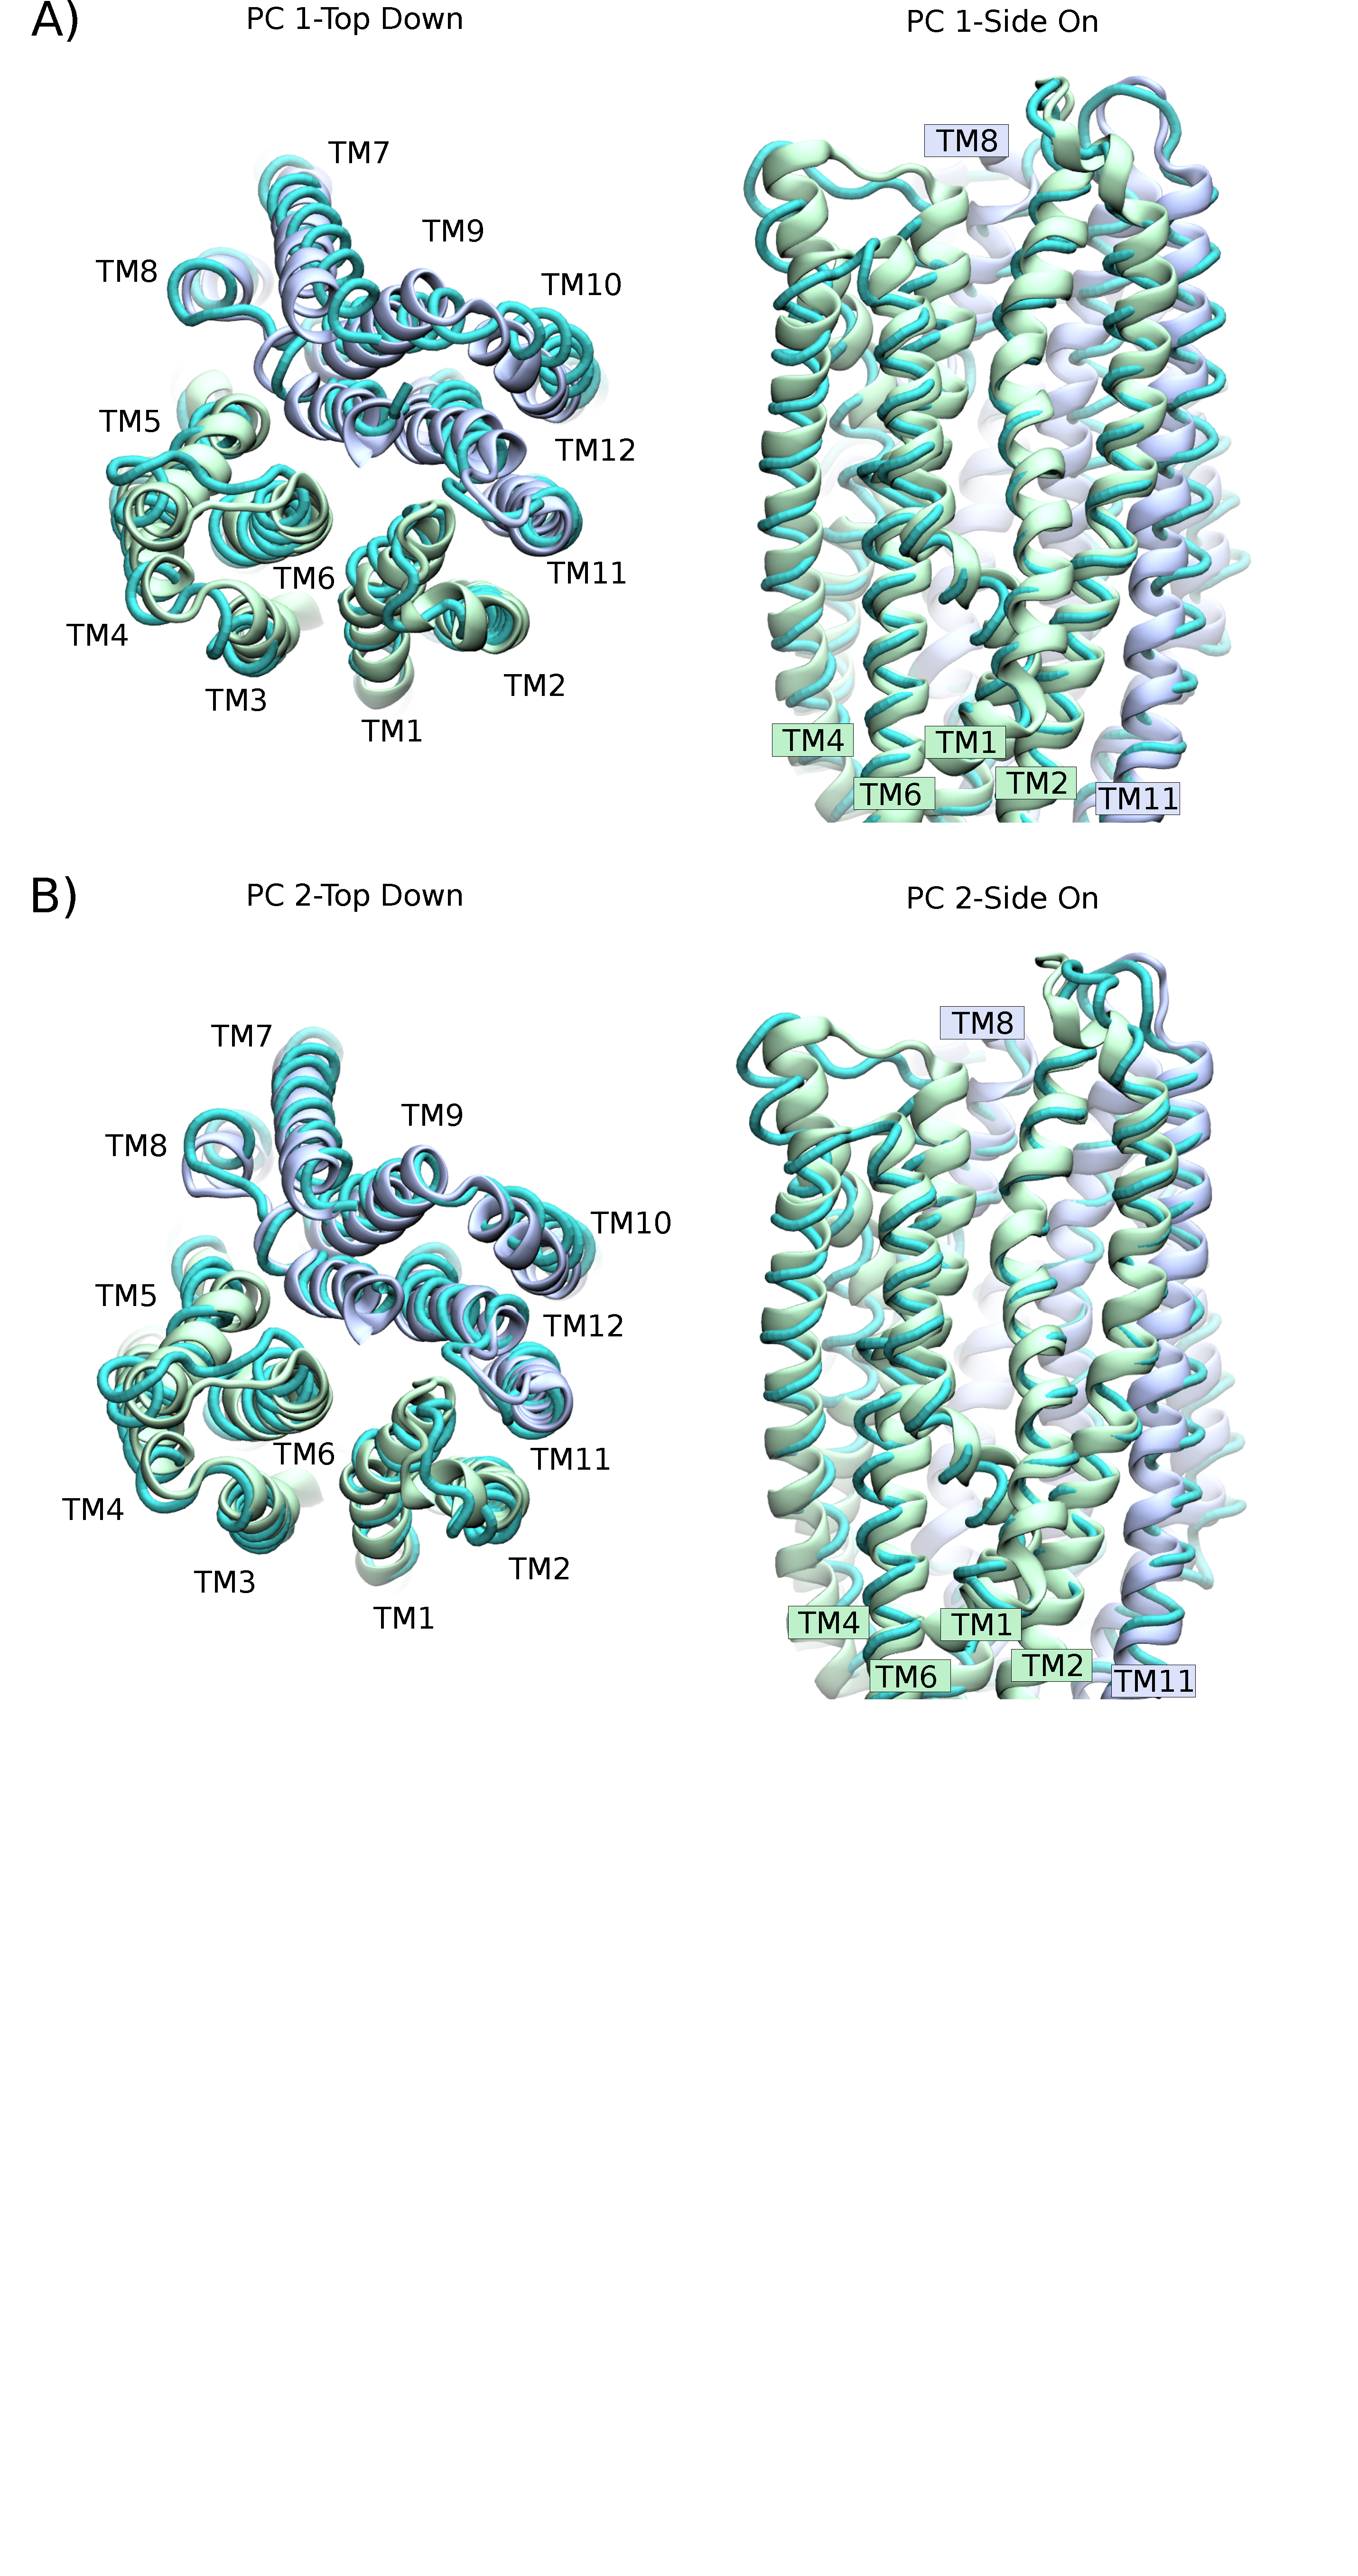
\includegraphics[width=1\textwidth]{figures/opening/pca_motions.pdf}
	\end{center}
	\begingroup
	\captionsetup{singlelinecheck = false, justification=raggedright}
	\captionof{figure}[Principal Component Analysis Reveals Large Motions in CFTR Transmembrane Helices] {\textbf{Principal Component Analysis Reveals Large Motions in CFTR Transmembrane Helices}}{A) Visualisation of the results from principal component analysis from 4 independent simulations, comprising 8.2 $\mu s$ of unbiased MD sampling. Motions along the first two principal component vectors were found to capture 38\% of the variation in the dataset and were used in further analysis. B) Visualisation of the first principal component vector (PC1). Note the motion in TMs 1, 6 and 8 C) Visualisation of the second principal component vector (PC2). Note the motions in TMs 1 and 6 but in directions orthogonal to PC1. A video has been rendered of the motions associated with PC1 and PC2 and can be accessed at the following \href{https://zenodo.org/record/7036443#.Yw7CZNJBwUE}{link}.\footnote{\href{https://zenodo.org/record/7036443\#.Yw7CZNJBwUEi}{https://zenodo.org/record/7036443\#.Yw7CZNJBwUEi}} D) Visualisation of the dilated open state which we will analyse in detail in subsequent sections. This structure was obtained by a linear combination of PC 1 and 2 followed by unbiased MD simulation. } 
	\label{PCA_motions}
	\endgroup

Since the more atoms we included in our collective variables, the slower our calculations would run, we limited subsequent free energy calculations to a set of helices directly surrounding the pore (Table \ref{red_alpha_carbons_table}) this is shown in Figure \ref{steer_cas_fig}. This was the same technique employed in \cite{hoffmann2018}. We later combined this choice of this choice of collective variables to discover an open conformation of CFTR. This revealed how the linear combination of PC1 and PC2 resulted in a stable, open conformation of CFTR which resulted from the displacement of TMs 1, 6 and 8 (Figure \ref{PCA_motions}D). 

\subsection{OPES-Metadynamics Finds a Stable Conformation with an Open Extracellular Pore}

The principal components derived in the previous section were used as collective variables to study the motion of the pore lining transmembrane helices in WT-CFTR. A two dimensional Free Energy Surface along these CVs was constructed through the use of 8 independent walkers, each running for $1.5\mu$s with On the Fly Probability Enhanced Sampling-metadynamics, using a barrier parameter of 38.2 kcal/mol (\ref{summary_FES}A). Convergence of these calculations is demonstrated in Figures \ref{convergence_opes_1}-\ref{convergence_3}. 

Note the presence of a local free energy minima at (0.010, 0.021) in Figure \ref{summary_FES}A. When this coordinate in CV space was investigated closely, we noticed that the extracellular pore had dilated significantly (Figure \ref{summary_FES}B). Further, this dilated configuration was stable in 3 replicates unbiased MD run for 500ns. 

This dilated structure has a pore architecture where the narrowest constriction was 2.8 $\angs$ (Figure \ref{summary_FES}C). This larger opening completely removed the aberrant constriction seen in the cryo-EM structure and the dilation occurred where we expected, between TM1 and TM6 (Figure \ref{summary_FES}D). Continuum models have previously estimated the constriction in CFTR to be of 2.4$\angs$ \cite{jun2016}. This is not far from our own estimate. 

	\begin{center}
		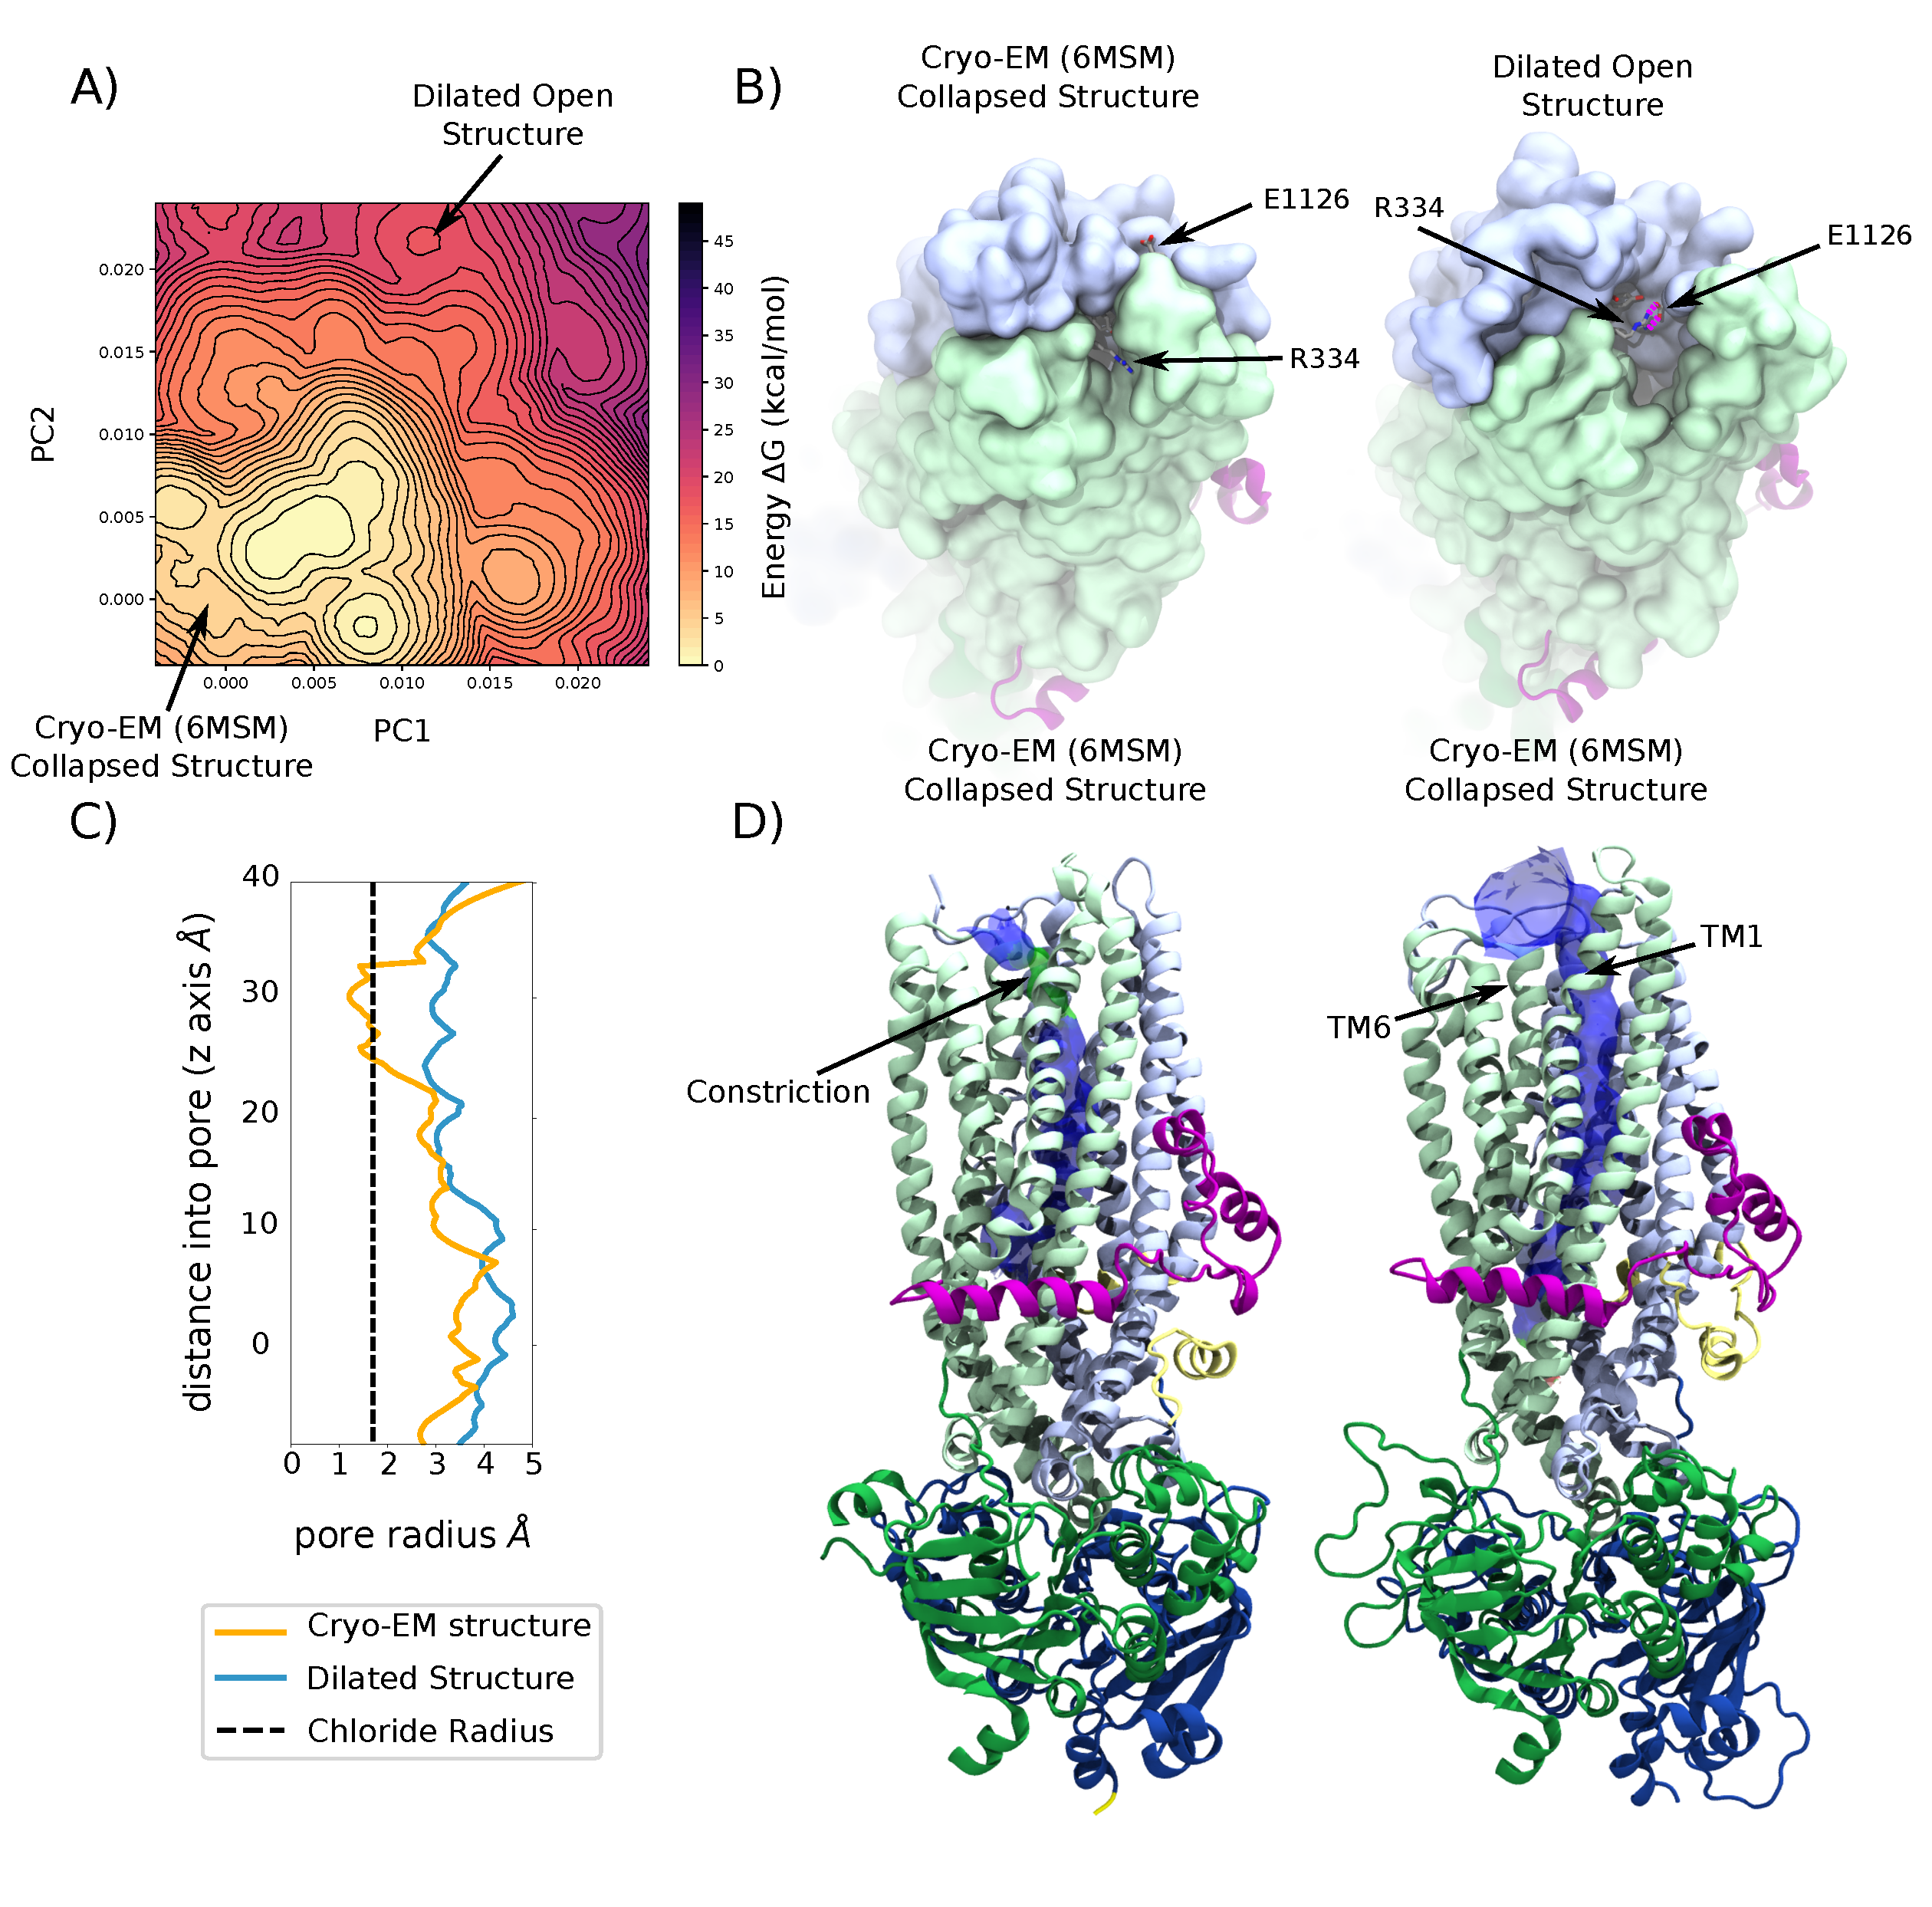
\includegraphics[width=1\textwidth]{figures/opening/summary_dilated_structure_1.pdf}
	\end{center}
	\begingroup
	\captionsetup{singlelinecheck = false, justification=raggedright}
	\captionof{figure}[Free Energy Calculations Discover a Dilated Conformation of CFTR.] {\textbf{Free Energy Calculations Discover a Dilated, Conformation of CFTR.}}{A) The free energy landscape obtained along PC 1 and 2 through OPES-Metadynamics. Note the free energy minimum corresponding to a collapsed structure, found cryogenic electron microscopy in the bottom left and the free energy minimum at (0.01,0.021). This latter well was found to correspond to a stable, open structure which appears capable of passing anions. B) A visual comparison between the constricted structure and our dilated open structure. Note how the extracellular opening is much wider in the dilated structure. The R334 and E1126 amino acids are visualised to show how they come into contact with each other in the dilated structure. C) A quantitative measurement of the pore radius for different conformations of CFTR, generated with HOLE2 \cite{smart1996}. Dehydrated chloride has a radius of 1.7 $\angs$, while the collapsed cryo-EM structure of hCFTR exhibits a constriction of 1.2 $\angs$. Hence, even if chloride were to be dehydrated during its migration through the selectivity filter, there would need to be some change to the surrounding protein conformation. By contrast, our proposed dilated open structure exhibits a constriction of 2.8 $\angs$ at its  narrowest point. This pore profile was generated from a snapshot obtained after 500ns of unbiased MD. Indicating that this open structure is energetically stable.  D) A side on comparison between the collapsed cryo-EM structure and the dilated open structure. The green constriction denotes the region too small to pass ions. This constriction has been completely removed in the dilated structure we have discovered. }
	\label{summary_FES}
	\endgroup


\subsection{The Open Conformation is Stabilised by the R334-E1126 Salt Bridge}
\label{salt_bridge}

In order to understand why the dilated open structure might be stable, we looked for interactions which would give rise to the free energy well in Figure \ref{summary_FES}A. We inspected pairs of positive and negative amino acids. Hence, a novel salt bridge was discovered, which linked R334 and  E1126. This salt bridge could only form in the dilated conformation, due to the movements of TM8 and TM6. It could not form in the collapsed cryo-EM structure (Figure \ref{salt_bridge_fig})A. 

This was possible due to the motions of TM1, TM6 and TM8. These movements allowing E1126 on ECL5 to come closer to R334 on TM6. We expect this new salt bridge to be an important determining factor in stabilising the conducting conformation of CFTR.  

The link between these amino acids was found to be stable in 3$\times$500ns unbiased MD simulations of the dilated structure. While it did not form at all in simulations of the cryo-EM structure (Figure \ref{salt_bridge_fig}B).

This is a novel interaction within CFTR which we have discovered through the use of simulations. Suggestions that this salt bridge exists can be found in the literature, but it has not been confirmed. We suspect this was due to the important role that R334 plays in conduction of anions and channel gating. We will discuss the implications of this salt bridge and the means for testing its presence \textit{in vitro} in the Discussion.

\begin{figure}
	\begin{center}
		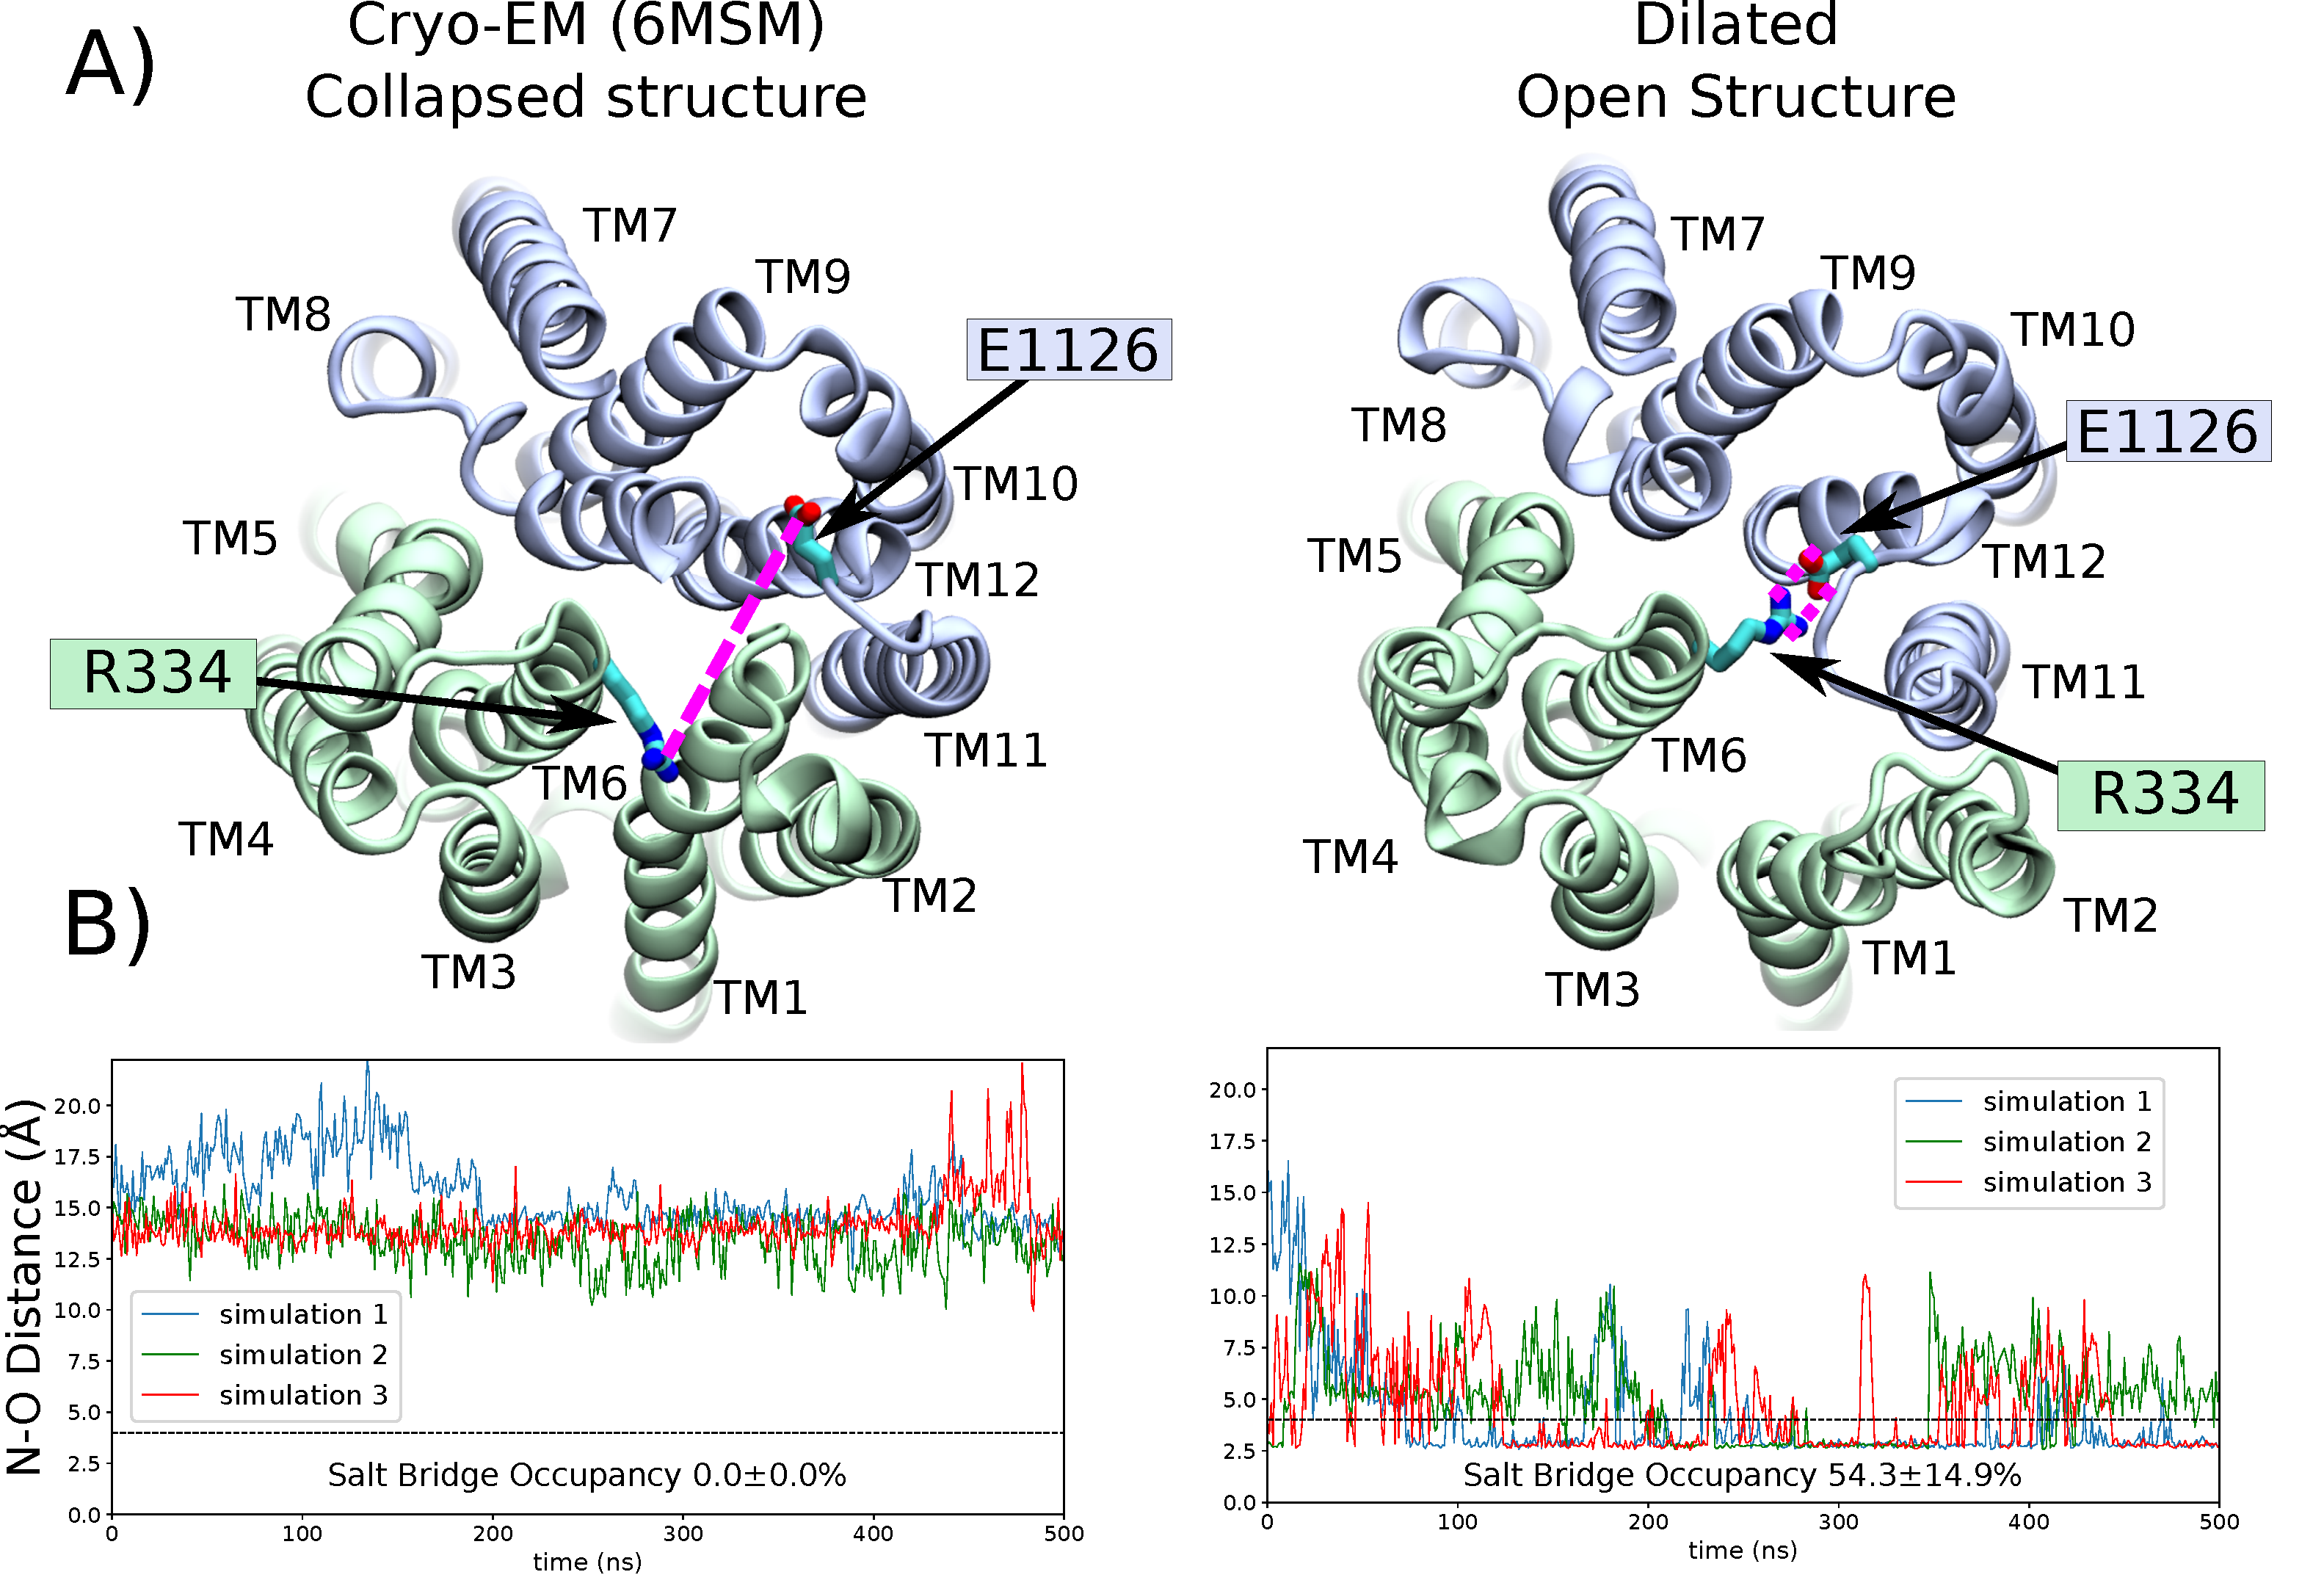
\includegraphics[width=1\textwidth]{figures/opening/salt_bridge_E1126_R334_figure.pdf}
	\end{center}
	\captionsetup{singlelinecheck = false, justification=raggedright}
	\caption[The Dilated Conformation of CFTR Gives Rise to the R334-E1126 Salt Bridge] {\textbf{The Dilated Conformation of CFTR Gives Rise to the R334-E1126 Salt Bridge}}{A) A comparison between cryo-EM and dilated CFTR structures. In the cryo-EM structure, R334 and E1126 are far apart and do not make contact. In the dilated structure, the transmembrane helices rearrange such that R334 and E1126 make contact. B) In simulations of the cryo-EM structure, the salt bridge is never formed. However, in the dilated structure R334 and E1126 come close together and form a stable salt bridge. The Dotted lines  in both plots denotes the distance below which the sidechains are in steric contact with each other. We believe that this salt bridge gives a significant energy contribution to the stability of the open channel. }
	\label{salt_bridge_fig}
\end{figure}

\subsection{Proving the Open Conformation is Capable of Ion Conduction with Umbrella Sampling}

In order to test the ability of the dilated structure to the conduct anions, we employed umbrella sampling to calculate the energy landscape of anions as they permeated through the selectivity filter of CFTR. 

The conduction of chloride through WT-CFTR in simulations of the cryo-EM structure was severely inhibited (Figure \ref{US_anions}A). We obtained a sizeable barrier of 9.7kcal/mol to the passage of chloride, demonstrating that without dilation, this structure will not allow chloride to pass at a rate in agreement with experiments \cite{gong2004}. By contrast, the dilated conformation obtained in the previous section removes steric barriers to the passage of chloride and larger anions (Figure \ref{US_anions}B). In this structure, a considerably smaller barrier of only 2.5 kcal/mol was observed for both chloride and the larger bicarbonate (Figure \ref{US_anions}C). 

This small barrier is closer to what we would expect to be overcome by the -46mV resting potential of epithelial cells \cite{josephson1979}. Furthermore, the remarkably similar profiles for both bicarbonate and chloride are in agreement with the energy landscape we would expect from a weakly selective channel like CFTR. Indeed, the umbrella sampling landscape has calculated the pathway through the ``permeability selectivity filter" of CFTR, a region where we the diffusion profile would differ between anions but not the energy landscape. Deeper in the pore is the ''conductivity selectivity filter", which we might expect to display a difference between the two anions. The lower FES in the vicinity of and R134 K95 in Figure \ref{US_anions}C for bicarbonate compared to chloride may indicate tighter binding at this site. This would lead to lower overall conductance of bicarbonate. Unfortunately, there have not as many studies which have measured the effect of mutations on bicarbonate conductance but studies of other anions would lead us to expect that R134 and K95 play an important role in the conduction of bicarbonate \cite{linsdell2016}. 

	\begin{center}
		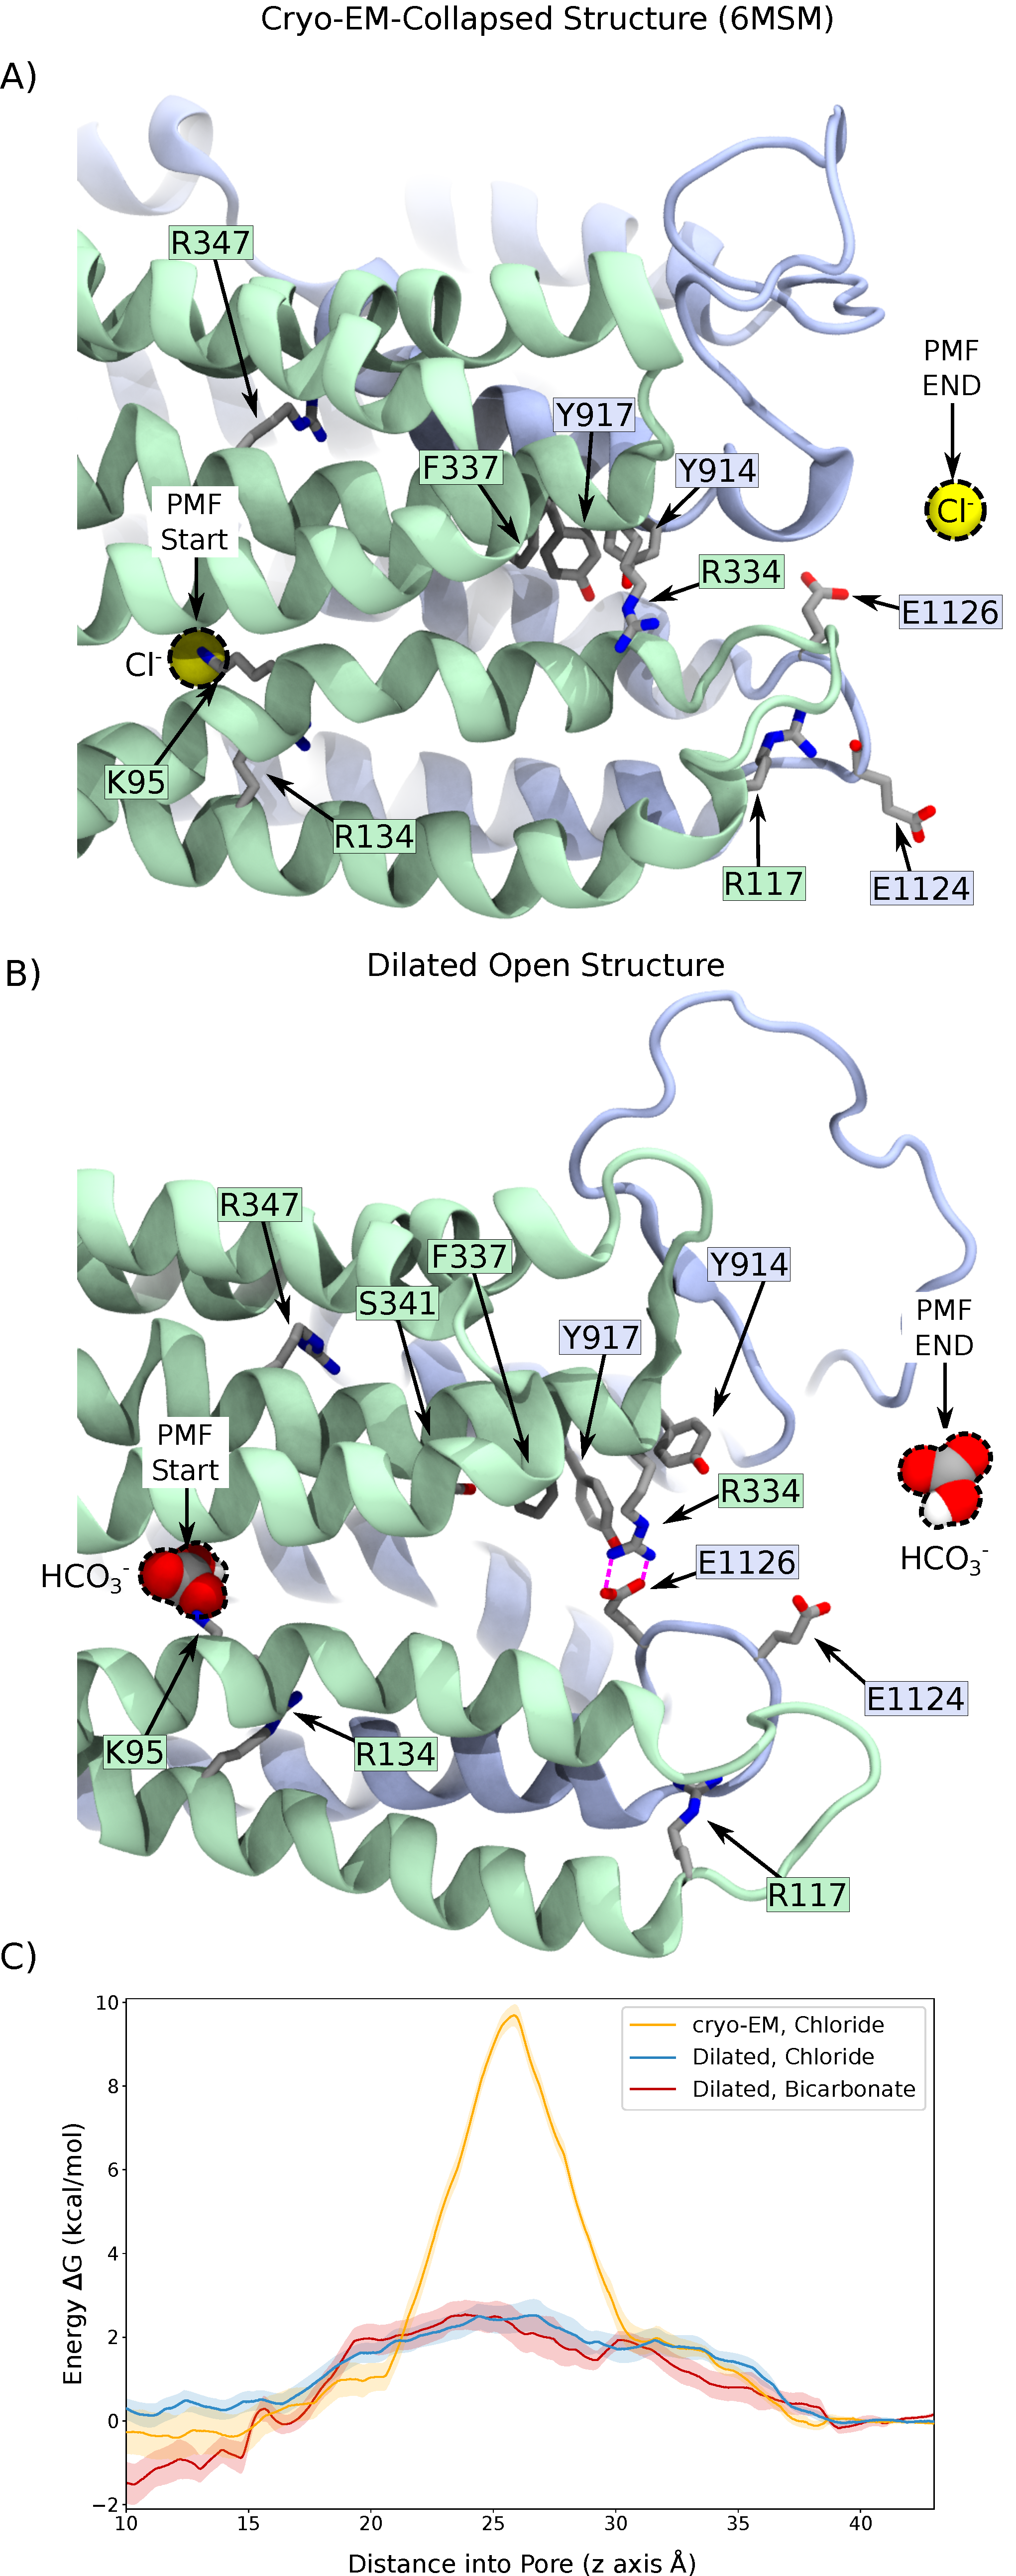
\includegraphics[width=0.6\textwidth]{figures/opening/pmf_fig_1_combined.pdf}
	\end{center}
\begingroup

	\captionsetup{singlelinecheck = false, justification=raggedright}
	\captionof{figure}[The Dilated Conformation of CFTR is Capable of Conducting Anions] {\textbf{The Dilated Conformation of CFTR is Capable of Conducting Anions}}{A) A close-up visualisation of the selectivity filter in the collapsed cryo-EM structure. To pass through this structure the ion must move past a tight constriction formed by F337, Y914 and Y917. B) A visualisation of the selectivity filter in our dilated \textit{in silico} structure. Here, bicarbonate is pictured but the same structure was used to construct a PMF of chloride as well. The selectivity filter is not as constricted and R334 can make a salt bridge with E1126. This brings R334 closer to the conduction pathway where it can help coordinate the permeating anion. Steric barriers to the conduction of anions have also been removed C) PMFs of the anions as they pass through the narrowest point in CFTRs permeation pathway. The collapsed cryo-EM structure exhibits a significant barrier to the conduction of chloride, this barrier is unphysically large and not what we expect given experimental measurements of this structure. By contrast, the dilated structure appears capable of permeating both chloride and bicarbonate, with a landscape in agreement with the characterisation of the channel found in experiments. }
	\label{US_anions}
	\endgroup



\subsection{The Open State Can be Used to Study Disease Causing Mutations in the Outer Pore, such as R334W}


\begin{figure}
	\begin{center}
		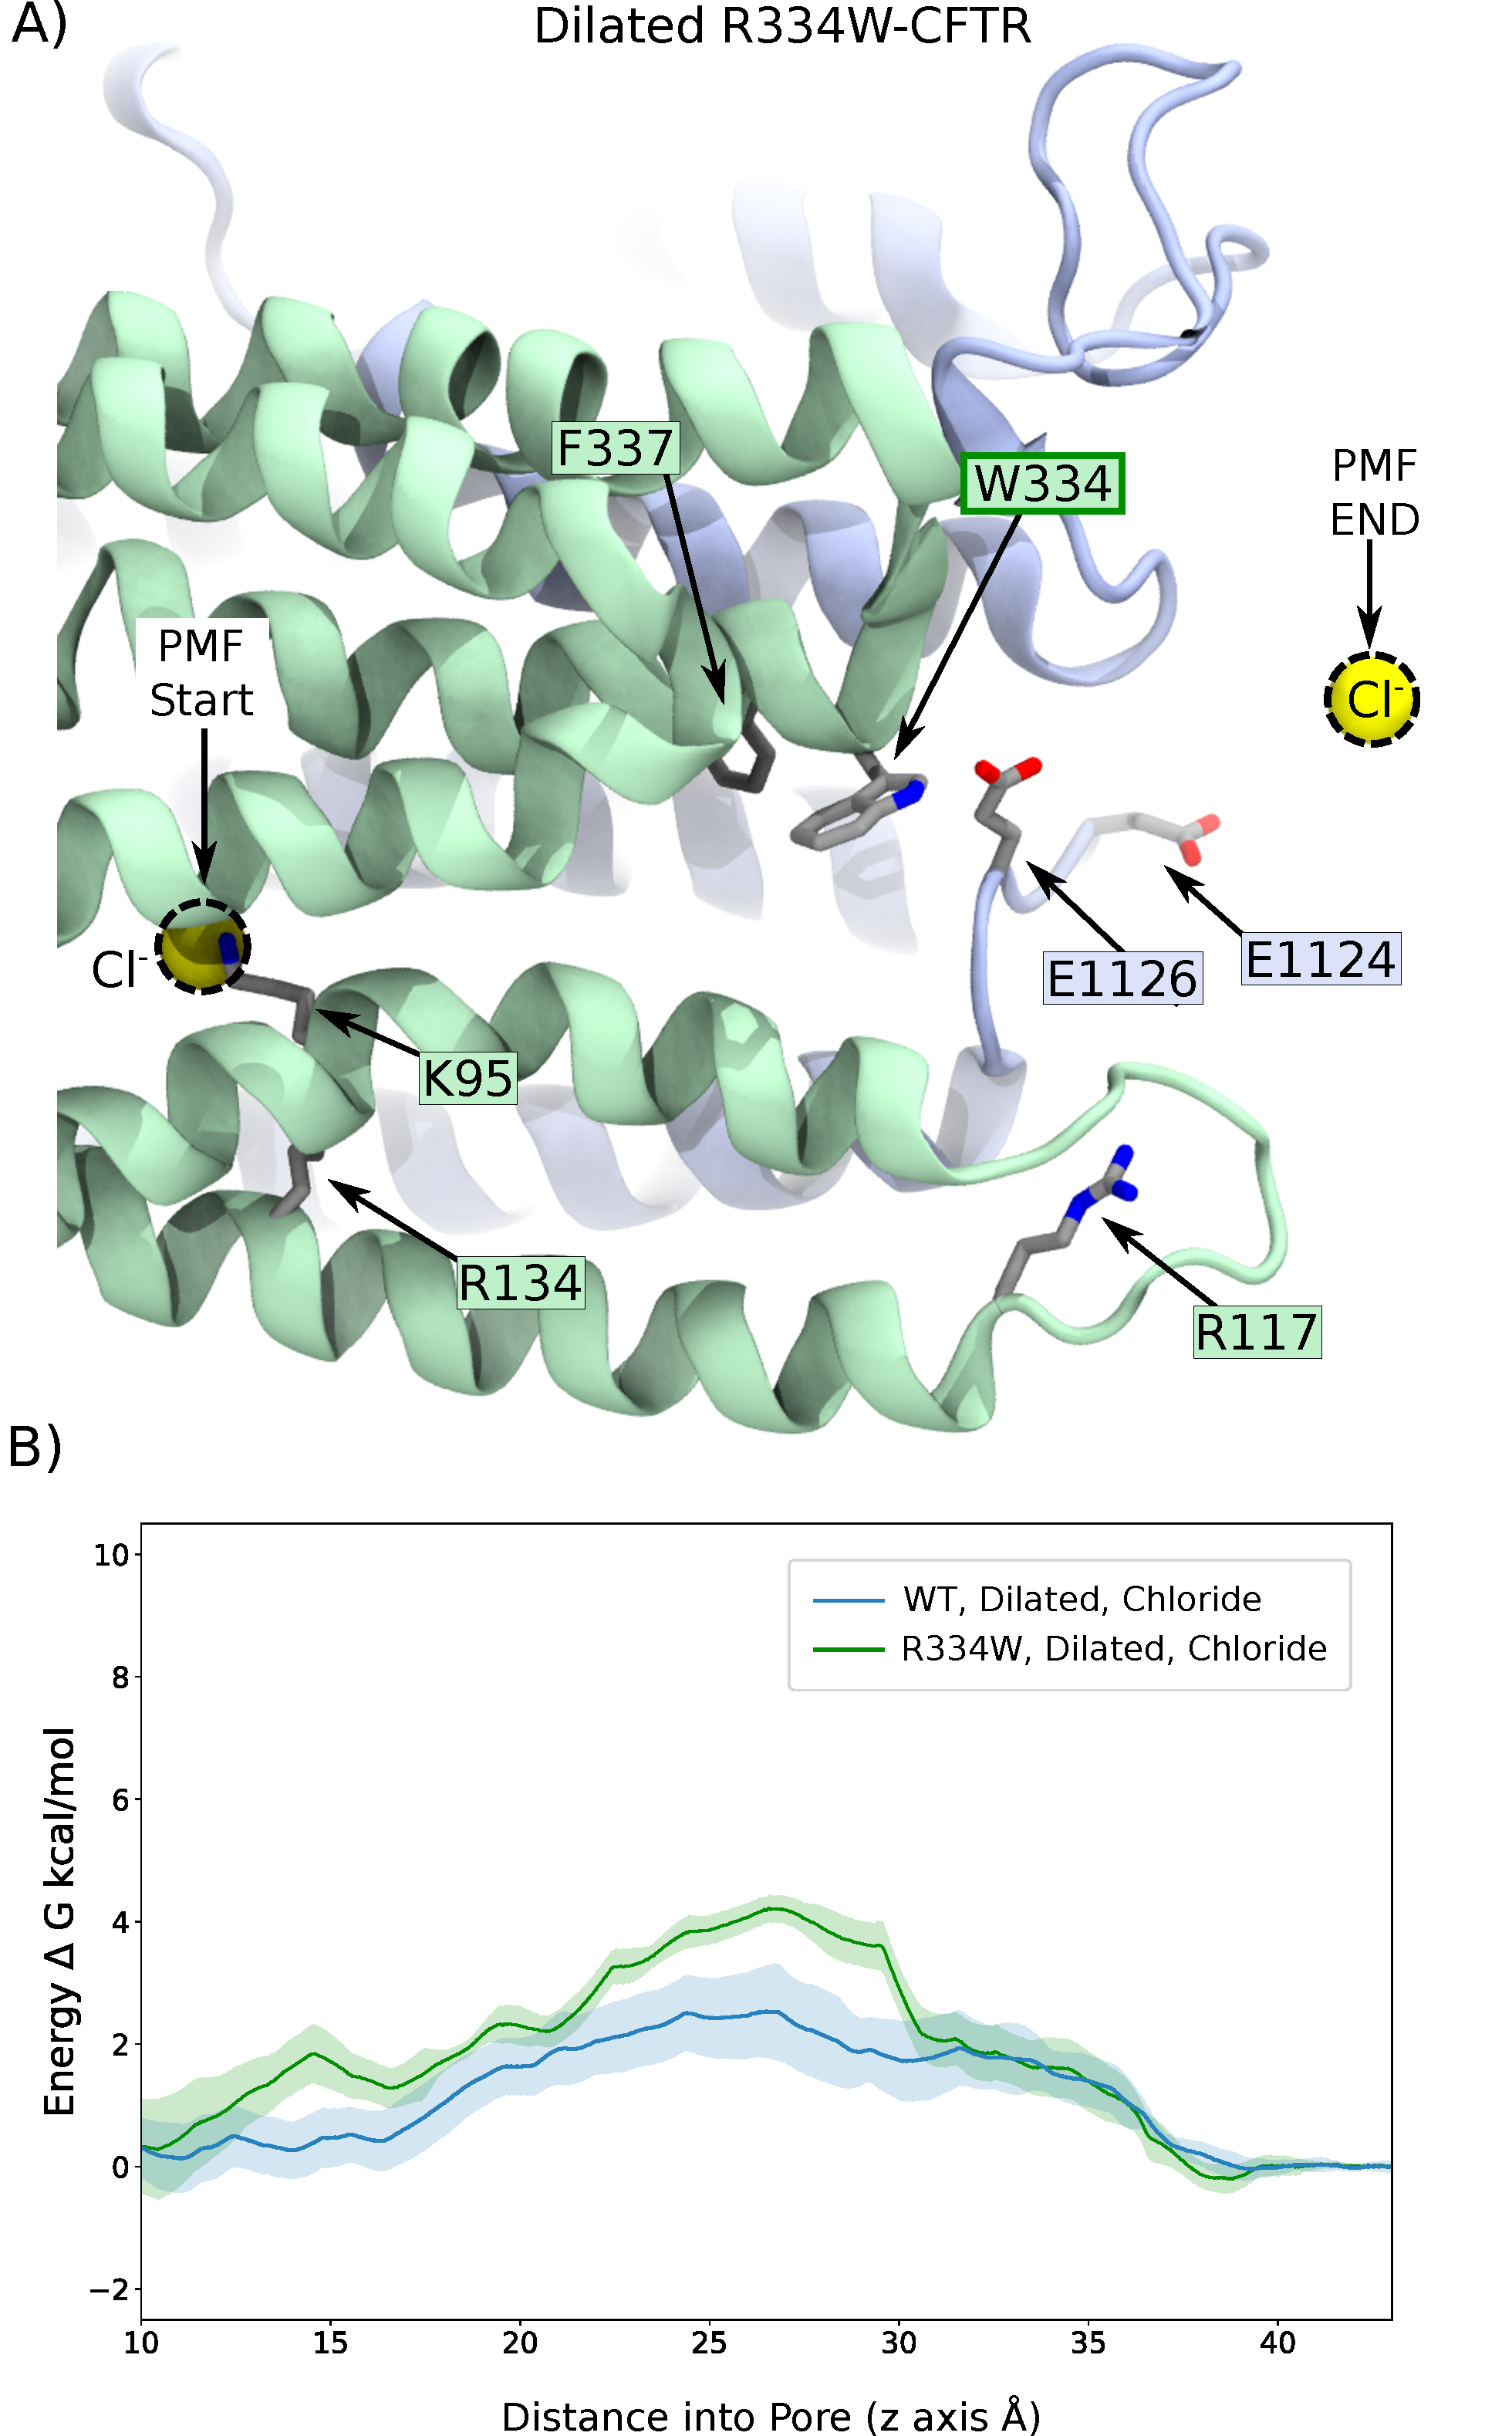
\includegraphics[width=0.6\textwidth]{figures/opening/R334W_pmf_combined.pdf}
	\end{center}
	\captionsetup{singlelinecheck = false, justification=raggedright}
	\caption[R334W Inhibits the Conduction of Anions] {\textbf{R334W inhibits the Conduction of Anions}}{A) A visualisation of R334W-CFTR in the dilated conformation. Note how W334 is placed in the outer part of the pore. B) A PMF derived from Umbrella sampling to compare the energetics of the conductance of chloride through R334W-CFTR to WT-CFTR in the dilated conformation. The WT-CFTR curve has been reproduced from the same data in Figure \ref{US_anions}C. The R334W-CFTR PMF exhibits a larger barrier compared to WT-CFTR indicating that the conduction of chloride will be inhibited in this mutation. It is likely that this additional energy barrier has a particularly deleterious effect on the conduction of the channel because it occurs at the narrowest part of the pore. There are no alternate pathways which might help compensate for the mutation, as was the case for R352Q in chapter \ref{chap:R352Q} \cite{wong2022a}.  }
	\label{R334_pmf}
\end{figure}

There are several disease causing mutations which occur at around the selectivity filter of CFTR (E116K, R334\{W,Q,L\},R117\{H,C,P\}, I336K, S341P)\cite{cftr2}. Note how these are all clustered around TM1 and TM6. The fact that mutations to these amino acids causes a loss of function is more evidence to suggest TM1 and TM6 form the permeation pathway for anions in hCFTR, as was found in previous MD and functional studies \cite{zeng2021,farkas2020, linsdell2016, linsdell2018}. 

A molecular understanding of these mutations can aid in the design of new therapeutics and so as an example, we used our dilated structure to study at the extracellular the R334W mutation. Single-ion channel studies of R334W-CFTR have found a current reduction of 60\% compared to WT-CFTR \cite{gong2004}. According to the Nernst-Planck model, this means we expect a larger energy barrier to the conduction of chloride in the mutant compared to WT-CFTR on the order of 0.6 kcal/mol \cite{kuyucak2001}. This is close to differences in barrier height we observed through umbrella sampling which were between 0.7 and 2.5 kcal/mol (Figure \ref{R334_pmf}B). 

\section{Discussion}

The present study diverges in an important way from recent \textit{in silico} investigations of large-scale conformational changes in ion channels. These past studies have focussed on recreating intermediate free energy landscapes between \textit{known} endpoints in conformational space \cite{lev2020, bergh2021, moradi2015}. These studies were \textit{targetted}. Such approaches are critical to the development of molecular techniques to help us understand the energetics and kinetics of protein systems. However, these techniques are inherently more limited by the availability of high quality experimental protein structures than \textit{untargetted} methods. So we present this \textit{untargetted} study as a proof of concept---to show how computational methods can move beyond the availability of protein structures.

One could regard the differences between \textit{targetted} and \textit{untargetted} MD methods as similar to the development of a unsupervised vs. supervised machine learning methods \cite{grus2015, friedman2017}. Each has its own advantages and drawbacks.

%The advantage of untargetted methods is that By using protein structures as a starting point, we can explore the conformational space around a region to understand more about a protein system. This has been made possible by increasing the increasing accuracy of protein forcefields to reproduce structural ensembles \cite{huang2016} and considerable increases to computer power. 


\subsection{The Dilated Structure Is Consistent with Experiments}
It is pleasing that the results from this chapter appear to correspond with results from \textit{in vitro} biophysical experiments. The movements in TM1 and TM6 which dominate the motions in PC1 and PC2 were the kind of dilation we expected from biophysical experiments of lone CFTR \cite{negoda2018}. \cite{negoda2019,linsdell2016}. The dilated structure also matches experiments which studied the binding of a protein partner WNK1 to TMD1 \cite{kim2019}. The dilation of the CFTR pore on the permeation of bicarbonate and other ions has been studied in detail \cite{jun2016, kim2019}. These studies indicate that movements of TM1 result in a wide open conformation, which facilitates the movement of bicarbonate ions.  

Additionally, the similar conductance profiles between bicarbonate and chloride are are the kind we would expect from a weakly selective anion channel like CFTR, particularly in the sampled region which corresponds to the ``permeability filter" \cite{linsdell2016}. Recall that the diffusion coefficient of a particle scales inversely with its radius according to the Stokes-Einstein relation \cite{miller1924}. Since chloride is smaller than bicarbonate we would expect it to permeate more quickly through the channel, even if it passed over the same energy landscape, particularly through the permeativity selectivity filter. 

Given that the conductivity ratio in CFTR is $P_{HCO3}/P_{Cl}=0.25$ the current, we would expect them to have a similar diffusion profile through the open channel. Indeed, the selectivity filter still as a constriction of 2.8 $\angs$, while a hydrated chloride ion has a radius of 3.2 $\angs$, so partial dehydration must still take place during anion conduction. Hence, our dilated conformation is still consistent with the experimentally determined lyotropic selectivity sequence found in other CFTR and other anion channels \cite{linsdell2016}. 

Cysteine cross-linking has been performed on many pairs of amino acids within CFTR \cite{negoda2019, cui2008, negoda2018, wang2012}. Our proposed conducting conformation is in close agreement with these studies, and in some cases, in closer agreement than the available cryo-EM structures. These studies found that the T338C/S1118C and R334C/T1122C cross-links could form in the open state but not in the closed state \cite{wang2012}. In the cryo-EM structure, TM8 stands in the way of these cross links. However, our dilated structure allows unobstructed access between TM6 and TM12, which would allow these cross-links to form. 

With the elucidation of CFTR in a conducting conformation, it may be possible to now design nano bodies or small molecules which select for it \cite{hutter2019}. This would give rise to to a new set of tools to understand CFTR's function or even new therapeutics to treat CF. Therapeutics which target the conducting conformation of CFTR will likely be much more effective than current generation potentiators which select for an open but not fully open conformation of CFTR \cite{csanady2019, yeh2017}. 

\subsection{Study Limitations}

We should address the considerable difference in height between the global free energy minimum in Figure \ref{summary_FES}A, which closely corresponds to the cryo-EM structure, and the minimum corresponding to our dilated structure. The dilated structure would appear to have a height of 17 kcal/mol. At first, this difference would seem unphysically high. If these values were correct, the dilated structure would be inaccessible at physiological temperatures. However, we believe this discrepancy is due to limitations of our simulation methods and we have plans to improve them. We believe there are 3 systematic issues which have lead to this discrepancy, outlining these issues will help us improve the study before submission for publication. 

The first and most pressing concern matter would be to improve our collective variables for OPES-MetaD. The PCA motions outlined in Figure \ref{summary_FES} are likely suboptimal. Note for example how in the dilated structure in Figure \ref{PCA_motions}D, TM1 has moved significantly but this motion is poorly captured by the two motions in Figure \ref{PCA_motions}A-B. Hence, the movement of TM1 is likely in a hidden CV, not captured by PC1 and 2 \cite{bussi2015, bussi2020a}. It is motions like this which have likely lead to some hysteresis during the construction of the free energy surface in Figure \ref{summary_FES}A. 

Given that the unbiased simulations of the dilated structure are stable, and they agree with experimental studies, we expect that the dilated state indeed corresponds to a physiologically relevant protein conformation. For the next iteration of this study, we plan to employ more advanced dimensionality reduction techniques such as TICA, VACs and RAVE to make a more careful choice of CVs \cite{brotzakis2019, noe2001, schultze2021, brotzakis2019, ribeiro2018}. We expect that the simple reweighing scheme of OPES-MetaD alongside SGOOP optimisation will be of great help in designing optimal CVs \cite{invernizzi2020, invernizzi2022, smith2018, tiwary2016b}. 

The second missing factor from the calculation of this FES is the energetic contributions from the anions as they pass through the selectivity filter. This is not captured by our CVs. The permeation pathway through CFTR is unusually long, and there has been a demonstrated energetic contribution from anions during channel gating \cite{gong2004, gong2003, gong2003a, tabcharani1993, zhou2002, sorum2015, yeh2015}. 

Finally, we consider the effects of the lipid bilayer which surrounds CFTR. There is emerging interest in the role played by the lipid bilayer in the regulation of CFTR and other membrane proteins \cite{cottrill2020, lin2022, kapoor2021, farinha2018, cui2020}. Different bilayer compositions have different physical properties, leading to different behavior by the proteins embedded in them \cite{hickey2011}. In the case of CFTR, many lipid species such as sphingolipids and cholesterol has been shown to lead to different rates of chloride transport, indicating that they play a role in regulating the gating of the channel \cite{aureli2016, farinha2018, cottrill2020}. Hence, it is likely that the zwitterionic POPC membrane used for these simulations will not reflect the energetics and kinetics of CFTR gating in its native environment.

The effect of the non-native lipid bilayer composition would also account for some discrepancies we find between our simulations and experiments. Careful biophysical experiments discovered an interaction between the R117 and the carboxyl atom of E1124 \cite{simon2021}. This interaction was not present in our dilated structure, nor was it well preserved in our unbiased simulations of the cryo-EM conformation (data not shown). Similarly, the well characterised R104-E116 interaction is poorly preserved in simulations of the cryo-EM structure and simulations of the dilated structure \cite{cui2014}. This discrepancy is also visible in previous MD studies of CFTR in a non-native lipid environment \cite{zeng2021}. These salt bridges were often broken in our MD simulations, due to interactions between the charged amino acids and the phosphate or choline chemical groups in the phospholipid bilayer. In future we could use newly developed model bilayers of the epithelium to simulate CFTR in a native-like environment \cite{wilson2021}. 

%Given the importance of different lipid species to regulation of CFTR such as cholesterol and sphingolipids, we expect that the zwitterionic POPC lipids used as a model membrane in this study do not fully reflect the native lipid environment of CFTR \cite{farinha2018, cottrill2020}. Recent studies have demonstrated an increasing need to study the bidirectional relationship between membrane composition and membrane protein regulation \cite{lin2022, kapoor2021, cui2020}. Hence, the state of the literature suggests that the salt bridges we mentioned earlier may in fact be regulated by the local environment of lipids around those specific sections of CFTR. 

We regard the above points as room for improvement, and they will be considered carefully in further studies of this dilated structure.

%Mutagenesis studies of the R334 amino acid noticed that many different mutations appear to result in ephys readings which would indicate a loss of function \cite{ge2004, gong2004, linsdell2021}. Surprisingly, the R334W mutation was determined not to alter the relative selectivity between anions in CFTR \cite{sheppard1993}. This is consistent with a wider open pore at the R334 position, as demonstrated in Figure \ref{summary_FES}.



%As shown by the results in the present study, the difficulty in converging a free energy landscape with collective variables derived \textit {ab initio} from long classical MD simulations can be difficult as the CVs are very likely going to be suboptimal. Machine learning techniques, more sophisticated than the simple PCA algorithm used here would likely do a much better job of choosing quickly converging CVs \cite{}. 

%The conformational changes investigated in this study occur within the lipid bilayer. This means that the kinetics and energetics of the transitions we have discovered will be highly dependent on the composition surrounding CFTR. It is well understood that the bilayer composition plays an important role in CFTR regulation and the clinical implications of this are an active area of research \cite{cui2020, cottrill2020}. It would therefore be an interesting study to repeat similar free energy calculations with different bilayer compositions to understand how they might regulate such conformational changes.


\subsection{Proposed Experiments to Test the R334-E1126 Salt Bridge}

The predictions of a stable salt bridge in section \ref{salt_bridge} fill a recent gap in the literature. The elegant study on the R117H mutation from Simon and Csanády \cite{simon2021} discovered that a long standing conclusion that R117 made a connection with E1126 was incorrect \cite{cui2014}. In fact, R117 makes a stable hydrogen bond with E1124, not E1126. This leaves the partner of the negative charge in E1126 unknown. The results from our dilation study would appear to fill this gap in the literature. There are some hints from previous biophysical studies to suggest that this salt bridge in fact forms \textit {in vitro}, and we will .

The critical role of E1126 to CFTR gating is demonstrated in Cui et al. \cite{cui2014}, while the most direct \textit{in vitro} suggestion of the formation of the R334-E1126 salt bridge comes from Wang et al. \cite{wang2016}. In this latter study, the researchers demonstrated that Zinc blocked the conduction of chloride through R334C-CFTR, indicating that zinc was binding at the extracellular mouth and blocking chloride. Because zinc has a charge +2$e$, they suspected that a nearby negative amino acid might might also play a role in binding the zinc cation. Further experiments showed conduction through the double mutant R334C/E1126A-CFTR was no longer inhibited by zinc ions. This lead the authors to suggest that R334-E1126 come close together in the open structure, forming a salt bridge. This is consistent with our \textit{in silico} findings which indicate that R334 and E1126 indeed form a salt bridge in the conducting CFTR conformation (Figure \ref{salt_bridge_fig}).  

It would have been very difficult to study the R334-E1126 interaction experimentally. This is because R334 plays such an important role in the conductance and gating gating of CFTR \cite{zhang2005,zhang2005a, gong2004, wang2012}. With the use of the atomic resolution offered by MD simulations, we have been able to fill this gap in the experimental literature, demonstrating the power of \textit {in silico} methods for studying protein dynamics. We propose that single ion channel patch clamp experiments measuring mutant CFTR could demonstrate the importance of the E1126-R334 salt bridge to the open state of the channel. 

Should the R334-E1126 play a role in stabilising the open channel, we would expect E1126 and R334 mutations to both exhibit a gating defect. There are already documented cases where mutations to these amino acids produce a gating defect and more careful investigations of these mutations would confirm the role of the R334-E1126 salt bridge in stabilising the open channel. A clear gating defect was observed in E1126R-CFTR \cite{cui2014}, while studies of R334C-CFTR found frequent transitions to a partially open state, with only infrequent transitions to a fully conducting state \cite{zhang2005a}. 

These results would lead us to expect that mutations like E1126A would have a similar gating phenotype to the R334C mutation. Should this be confirmed in experiments it would confirm the presence of our discovered R334-E1126 salt bridge in the conducting conformation of CFTR. If breaking both sides of this salt bridge results in the same phenotype, it would confirm that the two amino acids are in contact \textit{in vitro}. A double mutant such as R352C/E1126A-CFTR might make such studies easier, as the R352C mutation exhibits flickering phenotype which makes it possible to study the transient open states of CFTR and gain a more complete picture of its gating kinetics \cite{csanady2017, zhang2017b}. One could also use cysteine cross linking to study the double mutant R334C/E1126C or test the charge swapped mutant R334E/E1126R. If these constructs restore chloride transport, it would confirm the presence of the R334-E1126 salt bridge in WT-CFTR. However, this seems unlikely, given the sensitivity of CFTR to changes at the R334 position \cite{gong2004}. 

The role of R334 in the formation of this salt bridge would have previously been obscured in \textit{in vitro} experiments, because of the important role it plays in the gating and conductivity of CFTR \cite{gong2003, gong2004}. Hence, we have demonstrated the complimentary power of MD simulations to wet lab biophysical experiments. %Studies of R334C-CFTR have shown that \cite{zhang2005, rahman2013}. 

\subsection{The Open Structure is Important to the Study of Rare Mutations}

Our findings from this study tie into the broader theme of our work. In previous chapters we performed MD simulations to elucidate unique modes of CFTR misfunction and then shown that they are amenable to rescue by CFTR modulators. 

The simulations in this study helped us resolve the conductance defect exhibited by the R334W mutation and now we will search the literature for evidence that this defect can be rescued by CFTR modulators. It has been observed that despite a basal reduction in chloride transport of 98\% \cite{han2018}, R334W-CFTR function may still be restored by triple therapy in intestinal organoids \cite{vanwilligen2019}. Clinical trials currently underway to test whether these findings translate to better disease outcomes \cite{R334W_Euro_CF_trial}. Hence, the R334W mutation is another case where a unique molecular defect responds to CFTR modulators. The open structure we propose here will help in the study of other rare CF-causing mutations at the pore mouth, hopefully leading to better patient outcomes and the discovery of new therapeutics.


%.Due to computational restraints, we cannot yet directly observe the effects of small molecule to CFTR \textit{in silico}. Hence, we must appeal to \textit{in vitro} studies to determine whether the fingerprint of the molecular defect we discover through MD can be rescued by modulators. 

\section{Conclusion}
Here we have performed extensive Molecular Dynamics and Free Energy Calculations to study the permeation of chloride through the selectivity filter of CFTR. This was motivated by out standing questions surrounding the conduction mechanism of this anion channel, due to its constricted selectivity filter. By applying OPES-Metadynamics and umbrella sampling, we were able to demonstrate that a dilated conformation of CFTR is more capable of supporting the conduction of both chloride and bicarbonate. Further, we demonstrated how this dilated structure is in better agreement with experiments and how it can be sued to study rare disease causing mutations.

Through the careful study of our dilated open structure, we also discovered that a salt bridge between R334 and E1126 forms in the open structure, but not the collapsed cryo-EM structure. This led us to suggest single ion channel patch-clamp electrophysiology experiments which would confirm the presence of this salt bridge \textit{in vitro}. The confirmation of this open structure could lead to novel, more effective therapeutics.

The work in this chapter suggests that computational methods are now sufficiently developed such that creative application of MD simulations and enhanced sampling techniques can help complete our molecular understanding of proteins. Similar techniques to the ones employed in this chapter could be used in many protein systems. It is common for proteins to be imaged imaged very close to their active conformation, but during the imaging process they change conformation slightly \cite{bock2022}. Simulations could be be used to study these proteins in their active state. A limited but powerful example of this would be to further refine the methods applied in this chapter and then apply them to the partially collapsed structure of P-glycoprotein \cite{kim2018a}. This important structure could be dilated, in order to resolve the fully outward facing configuration, in a manner very similar to what we have done to CFTR.


%\textit {In vitro} studies of the state dependent formation of the extracellular helices of the distances between  TM1, TM6, and TM12 indicated that in the closed state these helices are tightly bound together (as can be seen in the 6MSM structure) and in the open state they move apart \cite{negoda2018}. Additionally, similar studies of TM8 demonstrate that Y914 and Y917 are solvent exposed, pore lining helices, position 914 linked to position 102 and 334 when they were each replaced by cysteines \cite{negoda2019}. The helical motions we see in our dilated structure are consistent with these experiments (Figure \ref{PCA_motions}D). 

%Mutations at R334 also exhibit a gating defect, with infrequent transitions to the fully open state \cite{zhang2005a ,cui2013a, sheppard1993}. However, the specifics of the burst kinetics of these mutations are understudied, likely because of the low conductivity of the R334W-CFTR channel which makes electrophysiology experiments difficult. This reveals the niche for simulations. Since we can offer atomic resolution into the dynamics of this channel, we can study the interactions in the mutant where it might be hard to do so experimentally. Multiple attempts were required to obtain an open structure of R334W-CFTR (data not shown). This raises the possibility that the open structure is less stable and the mutant may present a gating defect. It is likely that an involved path Metadynamics or string method with swarms of trajectories approach might reveal the pathogenic gating defect present in this mutation \cite{lev2020, hoffmann2018, branduardi2007}. Construction of such a protocol could be used to investigate other outer vestibule gating class defects such as R117H \cite{simon2021}.

\section{Methods Details}
\subsection{System Composition}
At a basic level, methodology used in this chapter is largely consistent with the other studies in this thesis with some key differences. The system was also constructed by embedding the extended CFTR model into a POPC membrane and then the whole these biomolecules were immersed in a neutralising 0.15 mol/L KCl solution. For all calculations in this chapter, except the initial unbiased calculations, the C-terminus was trunked at amino acid 1450 in order to make the simulation box smaller and save computer time.

\subsection{Unbiased MD }
The minimisation and equilibration steps for these simulations were largely carried out in the same way as for previous chapters. Our protein model was the extended CFTR model based on the 6MSM structure \cite{zhang2018} which we constructed in chapter \ref{chap:I37R}. The MD system was subjected to minimisation by steepest descent followed by restrained relaxation. This involved 10 kcal/mol $\angs^2$ harmonic restraints on all heavy protein atoms with restraints halved every 400 picoseconds. This relaxation was followed by up to 2.2 $\mu$s of unbiased molecular dynamics sampling.

\subsection {Principal Component Analysis and Choice of Collective Variables}
\label {supp_cv_choice}
Using principal component analysis on proteins can be difficult. PCA specialises in choosing the vectors which capture the \textit{largest} variation in a dataset. By contrast, when we are performing free energy calculations, where we would wish to capture the \textit{slowest} motions to accelerate \cite{noe2001}. 

So, when performing PCA on proteins, without excluding them, of large disordered loops would dominate the analysis. Hence, we limited our analysis to the amino acids in Table \ref{red_alpha_carbons_table}. The four unbiased trajectories were combined using \verb_gmx trjcat_, PCA was then performed using using \verb_gmx covar_ and finally the vectors were analysed and visualised using \verb_gmx anaeig_. The concatenation of the unbiased trajectories in this way is mathematically valid---as when PCA is solely performed 3d coordinates, it is agnostic to the temporal dimension of the data points \cite{grus2015}.

For the sake of performance, a smaller subset of amino acids were then chosen to actually manipulate the pore of CFTR in the OPES-Metadynamics simulations. These calculations were expensive and the more atoms included in our CVs the slower the calculations were run, so the amino acids highlighted in red in Table \ref{red_alpha_carbons_table} were chosen for further analysis. These were the pore lining amino acids and our choices closely reflect those of previous studies (Figure \ref{steer_cas_fig}) \cite{hoffmann2018}. 

There are two main disadvantages when using PC's as CVs. Firstly, as discussed, they correspond to the largest motion in a system, not the slowest. This means that they are very likely to be suboptimal CVs in a molecular system. Secondly, they are \textit{linear}. And so a linear combination of many PCs may be needed to find the minimum free energy pathway of a given transition. This gives rise to a trade off. The more CVs we have to consider during the free energy calculation, the more likely we are to find a minimum energy pathway, but the longer it will take to converge the FES. Benchmarking of our own calculations revealed that only 2 CVs could be used before the calculations slowed to unmanageable rates on available hardware. This led us to choose the first two PC's 1 and 2 from our analysis as the collective variables to accelerate in our enhanced sampling. These choices were made carefully. PCs 1 and 2 captured 38\% of the variance of the unbiased data, meaning they meaningful CVs, and they produced movements in TM1 and 6 in the directions we expected given the available biophysical evidence. 

	\begin{center}
	%\begin{tabular} {| c | c | c | c | c | c | c | c | c | c | c | c | }  
	\resizebox{0.85\textwidth}{!}{%
	\begin{tabular} {| c | c | c | c | c | c | c | c | c | c | c | c | }  
		\hline
		\textbf{TM1}  $\uparrow$ & \textbf{TM2}  $\downarrow$ & \textbf{TM3}  $\uparrow$ & \textbf{TM4}   $\downarrow$& \textbf{TM5}  $\uparrow$ & \textbf{TM6}   $\downarrow$& \textbf{TM7}  $\uparrow$ & \textbf{TM8}   $\downarrow$& \textbf{TM9}   $\uparrow$& \textbf{TM10} $\downarrow$ & \textbf{TM11}  $\uparrow$ & \textbf{TM12}   $\downarrow$\\ \hline

                         & 113                      &  218 & 219 &                          &                          & 885 &                          &                           & 1013 &                            &                           \\ \hline
                         & 114                      &  217 & 220 &                          &                          & 884 &                          &                           & 1014 &                            &                           \\ \hline
                         & 115                      &  216 & 221 &                          &                          & 883 &                          &                           & 1015 &                            &                           \\ \hline
                         & 116                      &  215 & 222 &                          &                          & 882 &                          &                           & 1016 &                            &                           \\ \hline
                         & 117                      &  214 & 223 &                          &                          & 881 &                          &                           & 1017 &                            &                           \\ \hline
112                      & 118                      &  213 & 224 & 330                      &                          & 880 &                          &                           & 1018 &                            & 1124                      \\ \hline
111                      & 119                      &  212 & 225 & 329                      & 331                      & 879 & 911                      &                           & 1019 &                            & 1125                      \\ \hline
110                      & 120                      &  211 & 226 & 328                      & 332                      & 878 & 912                      & 1012                      & 1020 & 1123                       & 1126                      \\ \hline
109                      & 121                      &  210 & 227 & 327                      & 333                      & 877 & 913                      & 1011                      & 1021 & 1122                       & 1127                      \\ \hline
\cellcolor{red!25}108 & \cellcolor{red!25}122 &  209 & 228 & \cellcolor{red!25}326 & \cellcolor{red!25}334 & 876 & \cellcolor{red!25}914 & \cellcolor{red!25}1010 & 1022 & \cellcolor{red!25}1121  & \cellcolor{red!25}1128 \\ \hline
\cellcolor{red!25}107 & \cellcolor{red!25}123 &  208 & 229 & \cellcolor{red!25}325 & \cellcolor{red!25}335 & 875 & \cellcolor{red!25}915 & \cellcolor{red!25}1009 & 1023 & \cellcolor{red!25}1120  & \cellcolor{red!25}1129 \\ \hline
\cellcolor{red!25}106 & \cellcolor{red!25}124 &  207 & 230 & \cellcolor{red!25}324 & \cellcolor{red!25}336 & 874 & \cellcolor{red!25}916 & \cellcolor{red!25}1008 & 1024 & \cellcolor{red!25}1119  & \cellcolor{red!25}1130 \\ \hline
\cellcolor{red!25}105 & \cellcolor{red!25}125 &  206 & 231 & \cellcolor{red!25}323 & \cellcolor{red!25}337 & 873 & \cellcolor{red!25}917 & \cellcolor{red!25}1007 & 1025 & \cellcolor{red!25}1118  & \cellcolor{red!25}1131 \\ \hline
\cellcolor{red!25}104 & \cellcolor{red!25}126 &  205 & 232 & \cellcolor{red!25}322 & \cellcolor{red!25}338 & 872 & \cellcolor{red!25}918 & \cellcolor{red!25}1006 & 1026 & \cellcolor{red!25}1117  & \cellcolor{red!25}1132 \\ \hline
\cellcolor{red!25}103 & \cellcolor{red!25}127 &  204 & 233 & \cellcolor{red!25}321 & \cellcolor{red!25}339 & 871 & \cellcolor{red!25}919 & \cellcolor{red!25}1005 & 1027 & \cellcolor{red!25}1116  & \cellcolor{red!25}1133 \\ \hline
\cellcolor{red!25}102 & \cellcolor{red!25}128 &  203 & 234 & \cellcolor{red!25}320 & \cellcolor{red!25}340 & 870 & \cellcolor{red!25}920 & \cellcolor{red!25}1004 & 1028 & \cellcolor{red!25}1115  & \cellcolor{red!25}1134 \\ \hline
\cellcolor{red!25}101 & \cellcolor{red!25}129 &  202 & 235 & \cellcolor{red!25}319 & \cellcolor{red!25}341 & 869 & \cellcolor{red!25}921 & \cellcolor{red!25}1003 & 1029 & \cellcolor{red!25}1114  & \cellcolor{red!25}1135 \\ \hline
\cellcolor{red!25}100 & 130                      &  201 & 236 & \cellcolor{red!25}318 & \cellcolor{red!25}342 & 868 & \cellcolor{red!25}922 & 1002                      & 1030 & 1113                       & \cellcolor{red!25}1136 \\ \hline
\cellcolor{red!25} 99 & 131                      &  200 & 237 & 317                      & 343                      & 867 & 923                      & 1001                      & 1031 & 1112                       & \cellcolor{red!25}1137 \\ \hline
 98                      & 132                      &  199 & 238 & 316                      & 344                      & 866 & 924                      & 1000                      & 1032 & 1111                       & \cellcolor{red!25}1138 \\ \hline
 97                      & 133                      &  198 & 239 & 315                      & 345                      & 865 & 925                      &  999                      & 1033 & 1110                       & 1139                      \\ \hline
 96                      & 134                      &  197 & 240 & 314                      & 346                      & 864 & 926                      &  998                      & 1034 & 1109                       & 1140                      \\ \hline
 95                      & 135                      &  196 & 241 & 313                      & 347                      & 863 & 927                      &  997                      & 1035 & 1108                       & 1141                      \\ \hline
 94                      & 136                      &  195 & 242 & 312                      & 348                      & 862 & 928                      &  996                      & 1036 & 1107                       & 1142                      \\ \hline
 93                      & 137                      &  194 & 243 & 311                      & 349                      & 861 & 929                      &  995                      & 1037 & 1106                       & 1143                      \\ \hline
 92                      & 138                      &  193 & 244 & 310                      & 350                      & 860 & 930                      &  994                      & 1038 & 1105                       & 1144                      \\ \hline
 91                      & 139                      &  192 & 245 & 309                      & 351                      & 859 & 931                      &  993                      & 1039 & 1104                       & 1145                      \\ \hline
 90                      & 140                      &  191 & 246 & 308                      & 352                      & 858 & 932                      &  992                      & 1040 & 1103                       & 1146                      \\ \hline
 89                      & 141                      &  190 & 247 & 307                      & 353                      & 857 & 933                      &  991                      & 1041 & 1102                       & 1147                      \\ \hline
 88                      & 142                      &  189 & 248 & 306                      & 354                      & 856 & 934                      &  990                      & 1042 & 1101                       & 1148                      \\ \hline
 87                      & 143                      &  188 & 249 & 305                      & 355                      & 855 & 935                      &  989                      & 1043 & 1100                       & 1149                      \\ \hline
 86                      & 144                      &  187 & 250 & 304                      & 356                      & 854 & 936                      &  988                      & 1044 & 1099                       & 1150                      \\ \hline
 85                      & 145                      &  186 & 251 & 303                      & 357                      & 853 & 937                      &  987                      & 1045 & 1098                       & 1151                      \\ \hline
 84                      & 146                      &  185 & 252 & 302                      & 358                      & 852 & 938                      &  986                      & 1046 & 1097                       & 1152                      \\ \hline
 83                      & 147                      &  184 & 253 & 301                      & 359                      & 851 & 939                      &  985                      & 1047 & 1096                       & 1153                      \\ \hline
 82                      & 148                      &  183 & 254 & 300                      & 360                      & 850 & 940                      &  984                      & 1048 & 1095                       & 1154                      \\ \hline
 81                      & 149                      &  182 & 255 & 299                      & 361                      & 849 & 941                      &  983                      & 1049 & 1094                       & 1155                      \\ \hline
 80                      & 150                      &  181 & 256 & 298                      & 362                      & 848 & 942                      &  982                      & 1050 & 1093                       & 1156                      \\ \hline
 79                      & 151                      &  180 & 257 & 297                      & 363                      & 847 & 943                      &  981                      & 1051 & 1092                       & 1157                      \\ \hline
 78                      & 152                      &  179 & 258 & 296                      & 364                      & 846 & 944                      &  980                      & 1052 & 1091                       & 1158                      \\ \hline
 77                      & 153                      &  178 & 259 & 295                      & 365                      & 845 & 945                      &  979                      & 1053 & 1090                       & 1159                      \\ \hline
 76                      & 154                      &  177 & 260 & 294                      & 366                      & 844 & 946                      &  978                      & 1054 & 1089                       & 1160                      \\ \hline
 75                      & 155                      &  176 & 261 & 293                      & 367                      &     & 947                      &  977                      & 1055 & 1088                       & 1161                      \\ \hline
 74                      & 156                      &  175 & 262 & 292                      & 368                      &     & 948                      &  976                      & 1056 & 1087                       & 1162                      \\ \hline
 73                      & 157                      &  174 & 263 & 291                      & 369                      &     & 949                      &  975                      & 1057 & 1086                       & 1163                      \\ \hline
 72                      & 158                      &  173 & 264 & 290                      & 370                      &     & 950                      &  974                      & 1058 & 1085                       & 1164                      \\ \hline
                         & 159                      &  172 & 265 & 289                      & 371                      &     & 951                      &  973                      & 1059 & 1084                       & 1165                      \\ \hline
                         & 160                      &      & 266 & 288                      & 372                      &     & 952                      &  972                      & 1060 & 1083                       & 1166                      \\ \hline
                         & 161                      &      & 267 & 287                      & 373                      &     & 953                      &  971                      & 1061 & 1082                       & 1167                      \\ \hline
                         & 162                      &      & 268 & 286                      & 374                      &     & 954                      &  970                      & 1062 & 1081                       & 1168                      \\ \hline
                         & 163                      &      & 269 & 285                      & 375                      &     & 955                      &  969                      & 1063 & 1080                       & 1169                      \\ \hline
                         & 164                      &      & 270 & 284                      & 376                      &     & 956                      &  968                      & 1064 & 1079                       &                           \\ \hline
                         & 165                      &      & 271 & 283                      & 377                      &     & 957                      &  967                      & 1065 & 1078                       &                           \\ \hline
                         & 166                      &      & 272 & 282                      &                          &     & 958                      &  966                      & 1066 & 1077                       &                           \\ \hline
                         & 167                      &      & 273 & 281                      &                          &     & 959                      &  965                      & 1067 & 1076                       &                           \\ \hline
                         & 168                      &      &     & 280                      &                          &     & 960                      &                           &      & 1075                       &                           \\ \hline
                         & 169                      &      &     & 279                      &                          &     & 961                      &                           &      & 1074                       &                           \\ \hline
                         & 170                      &      &     & 278                      &                          &     & 962                      &                           &      & 1073                       &                           \\ \hline
                         & 171                      &      &     & 277                      &                          &     & 963                      &                           &      & 1072                       &                           \\ \hline
						 &                          &      &     & 276                      &                          &     & 964                      &                           &      & 1071                       &                           \\ \hline
						 &                          &      &     & 275                      &                          &     &                          &                           &      & 1070                       &                           \\ \hline
            			 &                          &      &     & 274                      &                          &     &                          &                           &      & 1069                       &                           \\ \hline
						 &                          &      &     &                          &                          &     &                          &                           &      & 1068                       &                           \\ \hline
 
            



\end{tabular}%
}
\end{center}
\begingroup
\captionsetup{singlelinecheck = false, justification=raggedright}                           
\captionof {table}[Amino acids used to analyse and manipulate the outer pore of CFTR] {\textbf{Amino acids used to analyse and manipulate the outer pore of CFTR}}{All listed amino acids were included in the unbiased extraction of PCA components. The cells highlighted in red denote the amino acids which were used as collective variables to study the free energy landscape of PCA motions 1 and 2. These are visualised in Figure \ref{steer_cas_fig}. }

\label{red_alpha_carbons_table}
\endgroup

\begingroup
	\begin{center}
		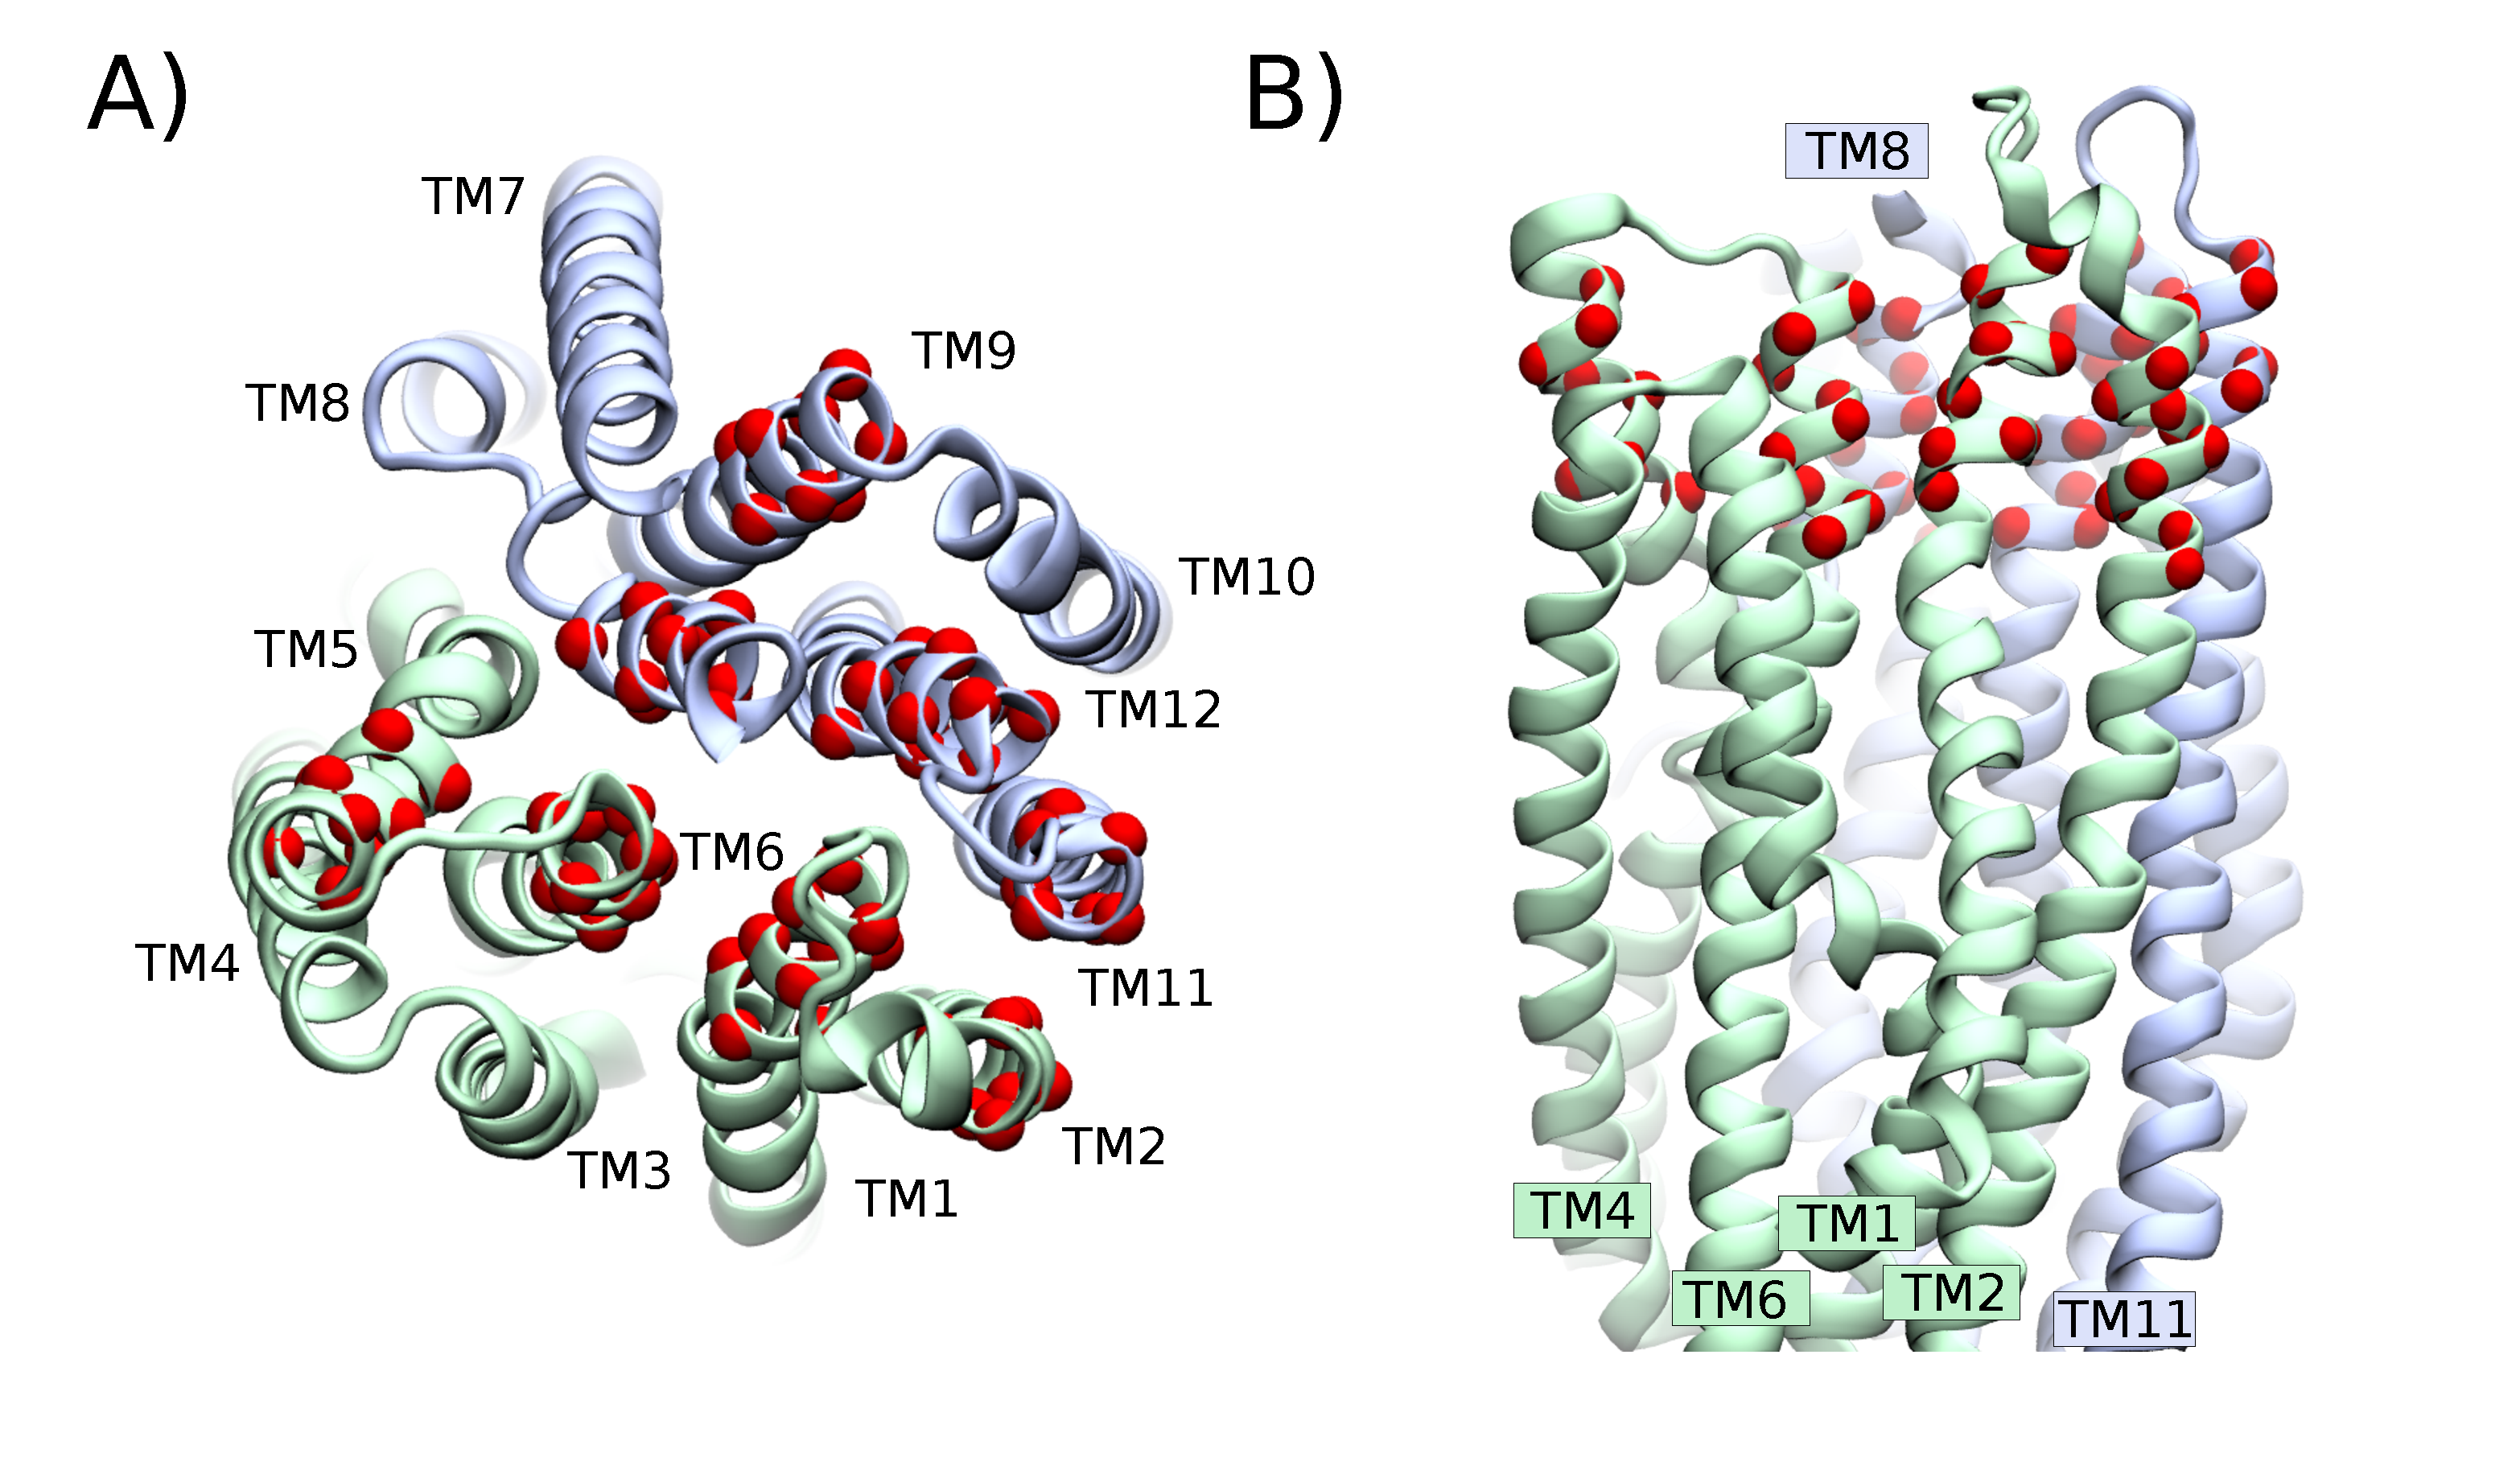
\includegraphics[width=1\textwidth]{figures/opening/steer_cas.pdf}
	\end{center}
	\captionsetup{singlelinecheck = false, justification=raggedright}
	\captionof{figure}[The Alpha Carbon Atoms Manipulated to Dilate CFTR] {\textbf{The Alpha Carbons Manipulated to Dilate CFTR}}{ The alpha carbon atoms represented as red spheres were pushed along PC1 and 2 during OPES-MetaD calculations. This allowed us to study the dilation of the CFTR pore. A) A top down view, note how pore lining helices have been selected for manipulation. B) A side-on view. Note how the upper section of the selectivity filter has been selected for manipulation. These choices of amino acids were made to prioritise the dilation of the extracellular mouth of the channel, which closely reflects the philosophy of a previous study \cite{hoffmann2018}. } 
	\label{steer_cas_fig}
\endgroup

%By selecting this subset, we applied Principal Component Analysis to the combined, aligned timeseries data from the alpha carbons of the amino acids in table \ref{pca_aas}. This allowed our analysis to focus on the slow, large motions which would most likely dilate the channel. The first 9 Principal Components were inspected visually. By the 4th vector, the motions were comparatively small and hence our analysis focussed on the first two motions. Motions 1 and 2 produced large movments in TM1 and TM6 which was where we expected the extracellular mouth to dilate. Hence, we chose to accelerate these first two motions.

\subsection{OPES-MetaD}
We employed 8 parallel walkers in order to properly explore and converge the free energy landscape along the two PC vectors discovered in the previous section. On the Fly Probability Enhanced Sampling with Plumed 2.8 was used to converge this difficult free energy landscape \cite{invernizzi2020, tribello2014}. Since we did not know exactly what kind of conformational change to expect and we had no \textit {ab initio} method to assess the quality of our CVs, a large barrier height of 38.2 kcal/mol was chosen for the OPES-MetaD protocol. This meant we could be confident that we would sample a large number of conformations. 

In order to decrease computational expense, masses were redistributed throughout the system using the conventional approach to Hydrogen Mass Repartitioning \cite{hopkins2015, balusek2019}. This allowed us to increase the simulation time step to 4 femtoseconds, while Gaussians were deposited every 2 picoseconds.

The free energy surface stopped evolving after each walker had run for 1500ns (Figures \ref{convergence_opes_1}-\ref{convergence_opes_2}). After this time multiple barrier crossings had been observed \ref{convergence_3}A.

One of the advantages of OPES-MetaD is that it provides simple variables which can be used to check the status of the simulation (Figure \ref{convergence_3}A-B). When the parameter 

\begin{equation}
	c(t) = \frac{1}{\beta} \log \langle e^{\beta V(t,\xi)} \rangle_\xi
\end{equation} 

plateaus, it is an indication that the FES has stopped evolving and the relative energetics of all points in the accessible CV volume have been estimated \cite{invernizzi2020, tiwary2015}. Here, $\beta=1/k_BT$ and $V(t,\xi)$ is the free energy estimate at time $t$. Similarly, we can check the volume of explored CV space with  

\begin{equation}
Z(t) = \frac{1}{| \Omega(t)|}  \tilde{P}(t, \mathbf{\xi}) d\mathbf{\xi}.
\end{equation} 

Here, $\Omega_n$ represents the volume of CV space explored which we use to normalise the probability estimate at time $t$ for a specific point in CV space $\tilde{P}(t, \mathbf{\xi})$. The convergence of $c(t)$ and $Z(t)$ in our free energy calculations is demonstrated in (Figure \ref{convergence_3}). Convergence of this parameter implies that the whole accessible CV volume at a given barrier parameter has been sampled Similarly, convergence of the $c(t) = \frac{1}{\beta} \log \langle e^{\beta V} \rangle$ parameter in Figure \ref{convergence_3}B indicates the free energy surface has stopped evolving and that the relative energetics of all coordinates in the accessible CV volume have been estimated.  

\begin{figure}
	\begin{center}
		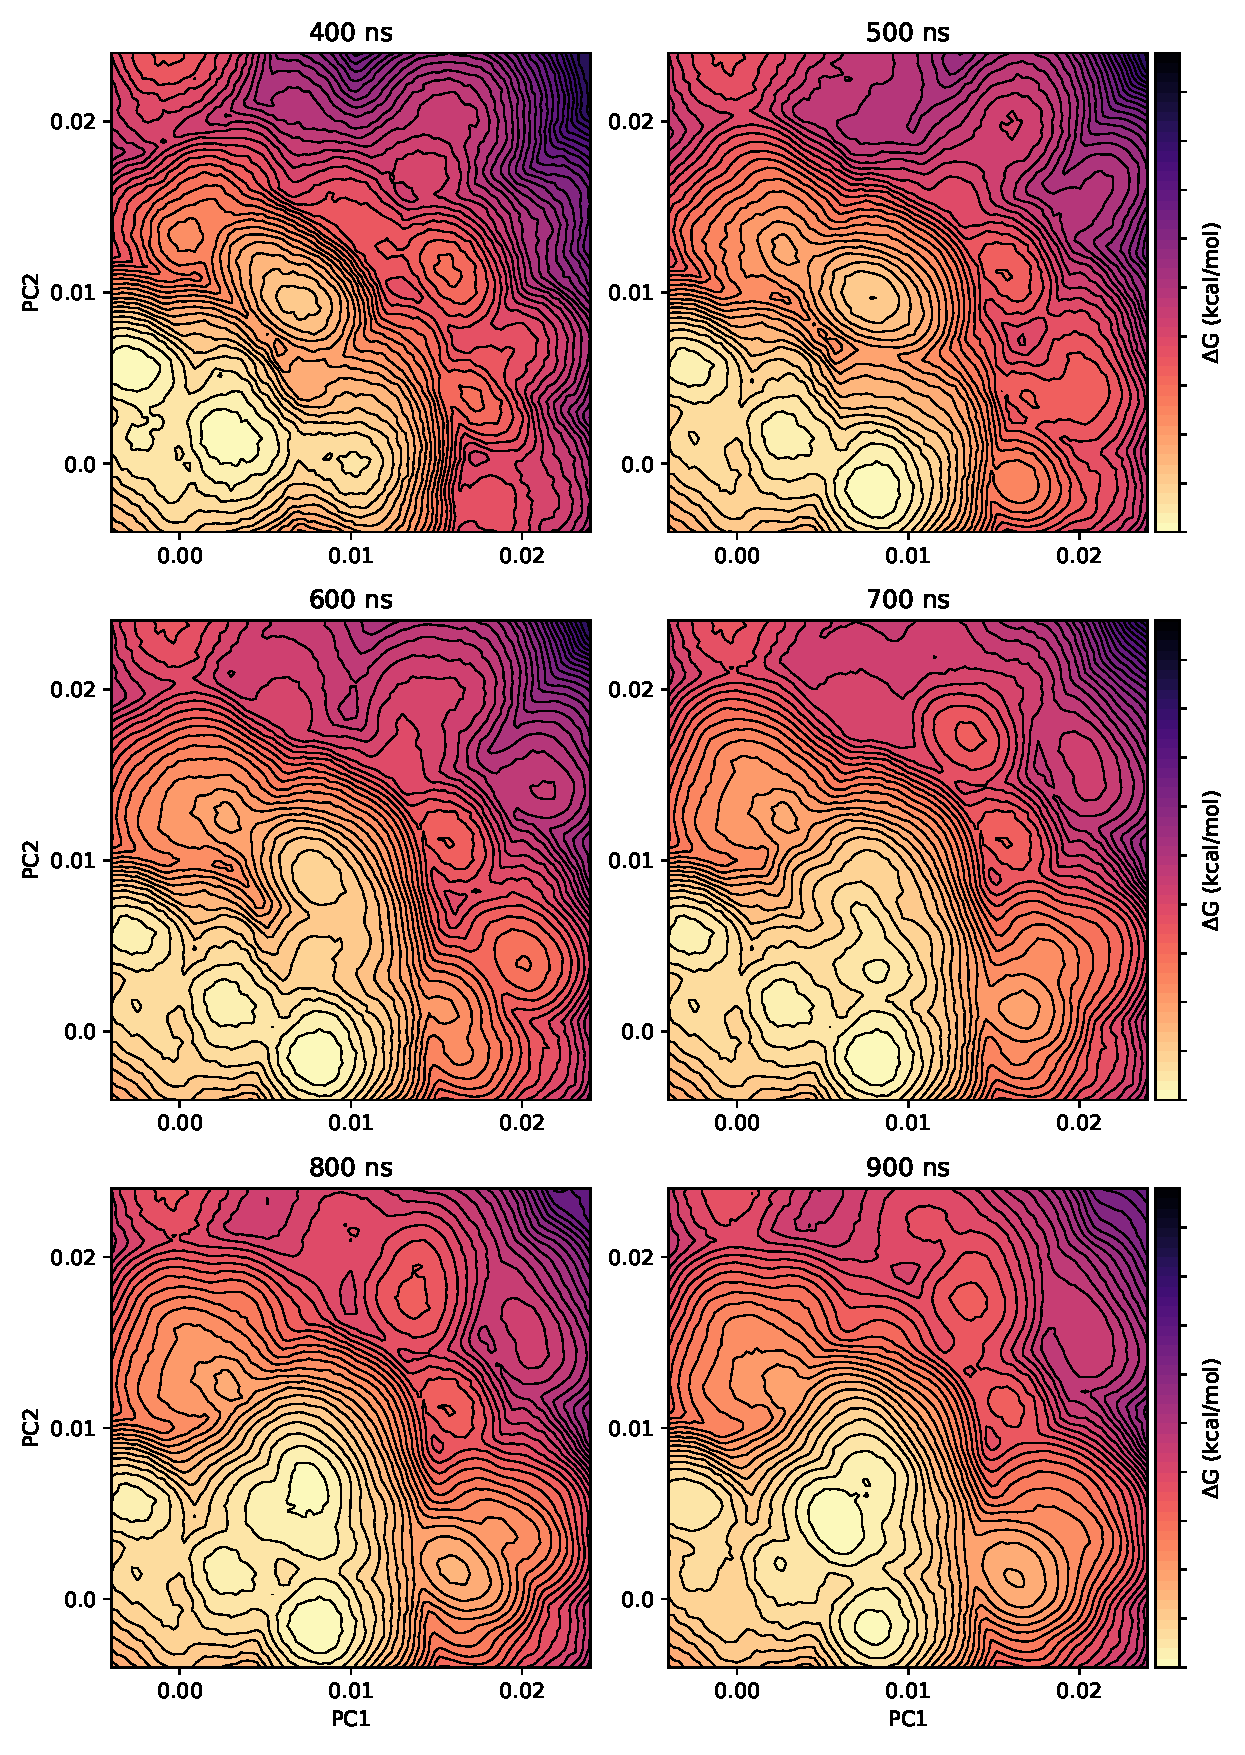
\includegraphics[width=0.8\textwidth]{figures/opening/convergence_1.pdf}
	\end{center}
	\captionsetup{singlelinecheck = false, justification=raggedright}
	\caption[OPES MetaD Free Energy Surfaces 400ns-900ns] {\textbf{OPES MetaD Free Energy Surfaces 400ns-900ns}}{The surface nearest to the cryo-EM starting point converges first.} 
	\label{convergence_opes_1}
\end{figure}

\begin{figure}
	\begin{center}
		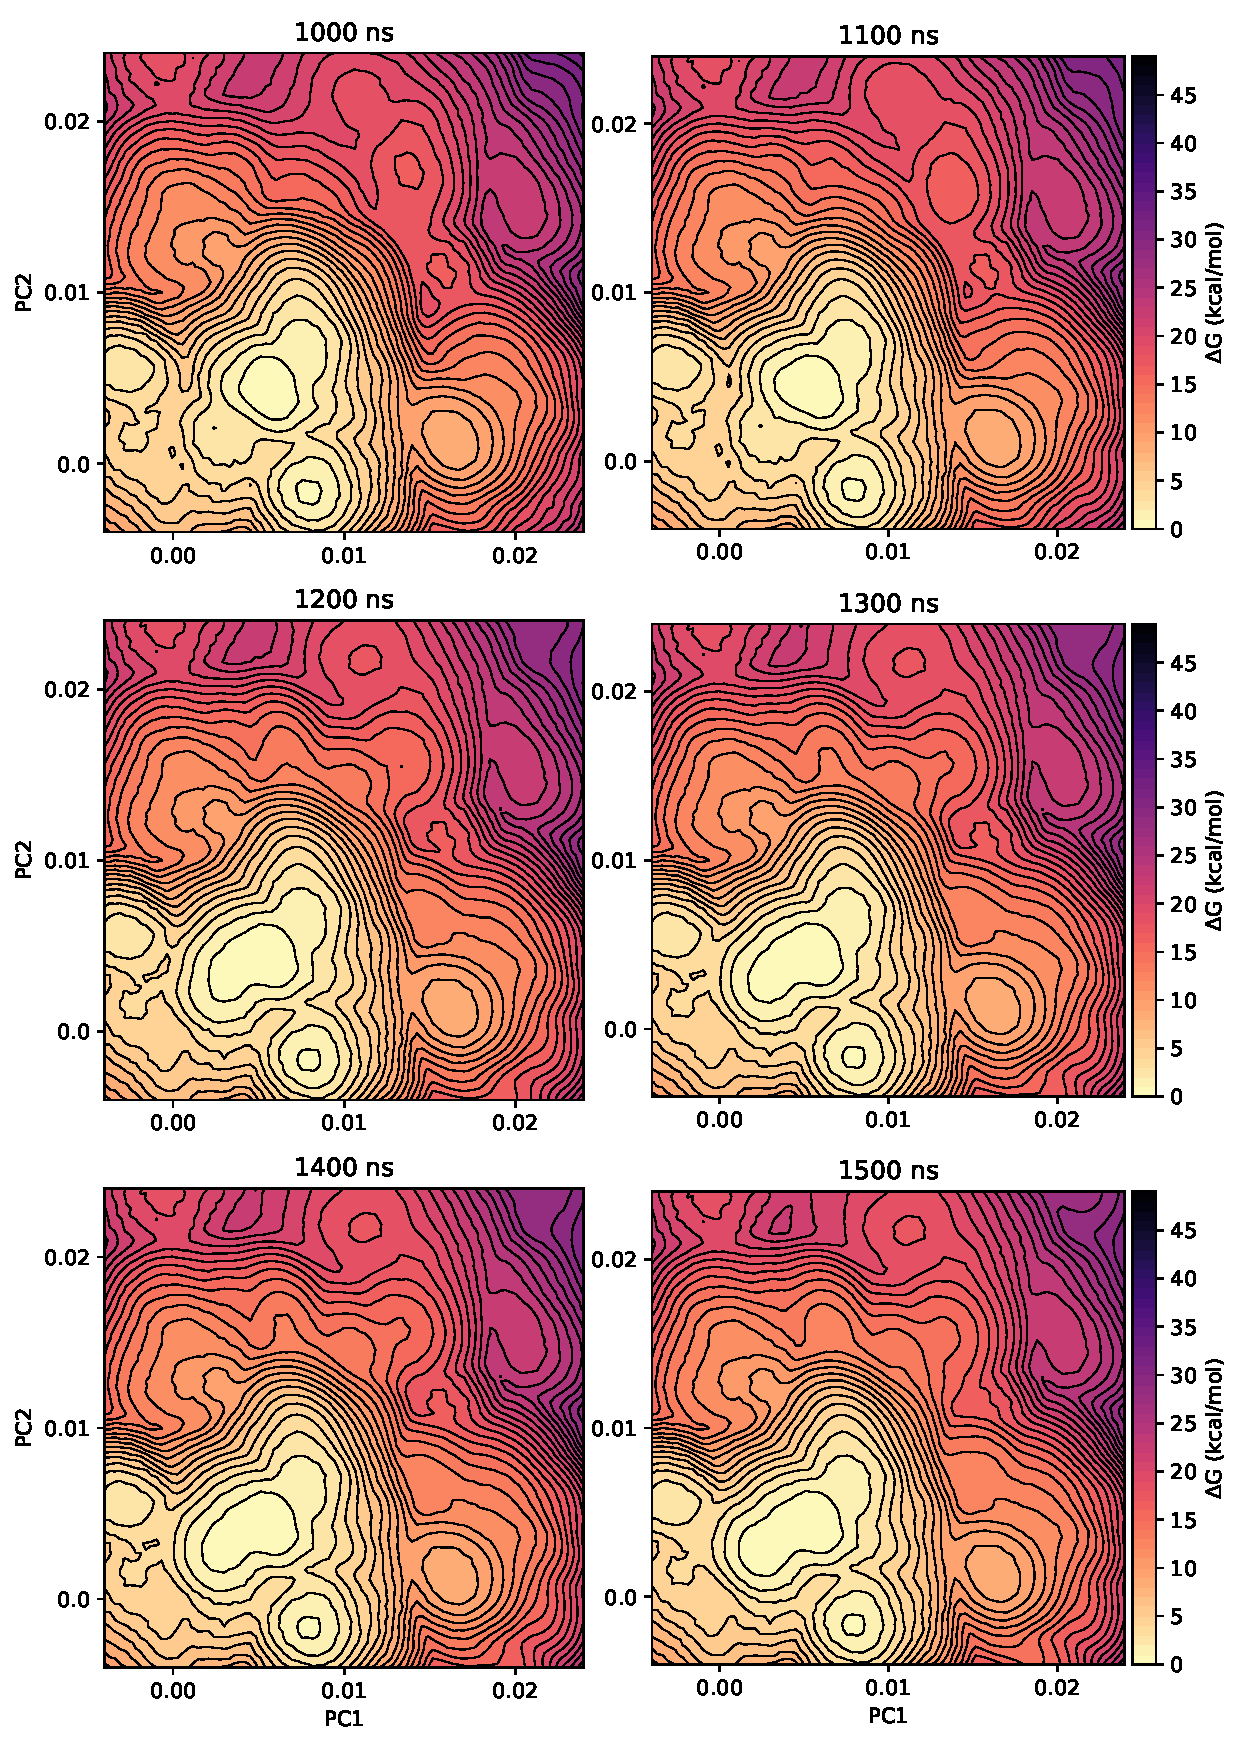
\includegraphics[width=0.8\textwidth]{figures/opening/convergence_2.pdf}
	\end{center}
	\captionsetup{singlelinecheck = false, justification=raggedright}
	\caption[OPES MetaD Free Energy Surfaces 1000ns-1500ns] {\textbf{OPES MetaD Free Energy Surfaces 1000ns-1500ns}}{Observe how by the last two surfaces are nearly identical. } 
	\label{convergence_opes_2}
\end{figure}

\begin{figure}
	\begin{center}
		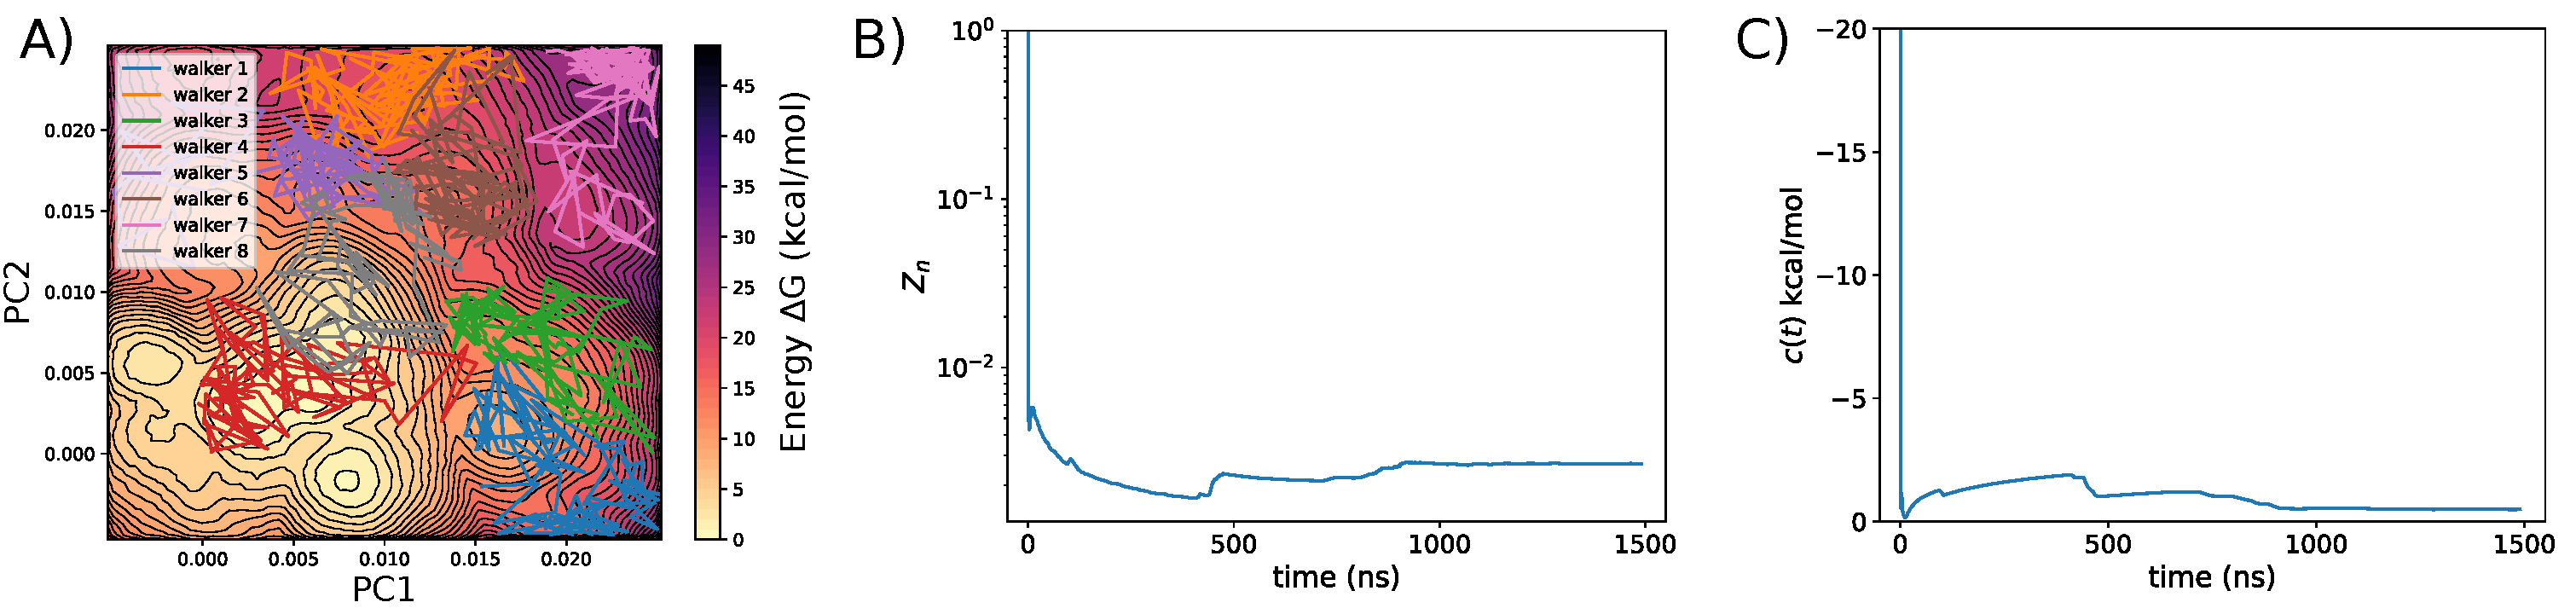
\includegraphics[width=1\textwidth]{figures/opening/FES_mw_trace.pdf}
	\end{center}
	\captionsetup{singlelinecheck = false, justification=raggedright}
	\caption[Demonstration of OPES-MetaD Convergence ] {\textbf{Demonstration of OPES-MetaD Convergence}}{A) The last microsecond of sampling for the 8 walkers in the OPES-MetaD simulations. Results indicate several barrier crossings between the constricted cryo-EM conformation in the bottom left region and the dilated open conformation studied in detail in the results section, indicating convergence. Somme sections of the landscape appear to be under sampled and so we recommend a more careful choice of CV in future. B) A graph of the $Z_n$ parameter from the OPES-MetaD calculation. These results indicate that the available CV volume has been sampled in the calculation. Note the log scale on the y-axis. C) The $c(t)$ parameter from the OPES-MetaD calculation. These results indicate that the calculation has converged and the FES has stopped evolving. }
	\label{convergence_3}
\end{figure}

\subsection{Assessing the Stability of the Dilated Conformation}
To test the stability of the dilated structure, restraints on PC1 and PC2 were slowly introduced to the WT-CFTR structure. Over the course of 5 ns harmonic restraints were added centered at (0, 0)-This corresponds to the location in CV space of the cryo-EM structure. The centers of these harmonic restraints were then steered to the location of the discovered local minima in CV space (0.010, 0.021) over the course of 10ns. The structure was allowed to equilibrate, while restrained at this location for 50ns. The restraints were slowly released over the course of 15ns. An equilibration period with no restraints was allowed for  unbiased MD was then run for 500ns.

A similar protocol was used to investigate the other free energy minima in Figure \ref{summary_FES}A. However, these did not produce a dilated structure, rather they exhibited constrictions similar to the cryo-EM structure and so they have not been analysed here in detail.

\subsection{Umbrella Sampling}
All Umbrella sampling studies were carried out with the same methodology. In all the unbiased equilibration steps of a CFTR simulation, an anion was found to spontaneously occupy the inner vestibule. This was selected as the ion to steer through the channel in the umbrella sampling

The collective variable in each US simulation was constructed by calculating the z coordinate of the center of mass of the alpha carbon atoms of all the amino acids in Table \ref{red_alpha_carbons_table} and then subtracting the z position of the steered anion. Meanwhile, the radial position of the ion was restrained a half potential well, when the ion strayed more than 4.8 $\angs$ from the center axis of the CFTR channel it would encounter a repulsive 10kcal/mol $\angs^2$ harmonic potential. This meant the ion could not stray too far from the center axis of the channel in bulk solvent but while it was inside the channel it could adequately sample the interior of the selectivity filter.

In order to calculate the PMF through the channel, we steered this anion to the middle of the channel ($Z=20\angs$) over the course of 10ns and allowed it to equilibrate there for 20 ns. The anion was then steered to its target location in a given window over the course of 10ns. It was then allowed to equilibrate at the target location for 10 ns before a 50ns production run. Windows were spaced 1 $\angs$ apart, meaning each PMF consisted of 40 windows.

To calculate the PMF through the selectivity filter we recorded the Z coordinate every picosecond for 50ns. The Weighted Histograms Analysis Method (WHAM) was then used to process the data from each window \cite{grossfield2012}. Independent PMF profiles of each CFTR system was then aligned at their extreme end ($Z=42-48\ \angs$), which corresponded to the flat energy surface obtained from pulling pulling an ion through bulk solvent. This gave us an absolute reference point to compare between different CFTR systems. 

To calculate uncertainties, the data from the production run was binned into 5 independent blocks of 10 nanoseconds, and an individual PMF was constructed for each of these blocks. The uncertainty was then given by doubling the Standard Error of the Mean between these 5 independent samples. Note how the uncertainties are below 1 kcal/mol across all PMFs in Figures \ref{US_anions} and \ref{R334_pmf}, indicating that the calculations had converged.

No restraints were placed on the architecture of the transmembrane helices during the umbrella sampling, demonstrating that they were in a stable conformation. 
